\documentclass[12pt, oneside]{book}

\usepackage[utf8]{inputenc}
\usepackage[spanish, es-lcroman, es-tabla]{babel}
\usepackage{csquotes}
\usepackage{graphicx}
\usepackage{subcaption}
\usepackage{tabularx}
\usepackage{longtable}
\usepackage{adjustbox}
\usepackage{amsmath}
\usepackage[hidelinks]{hyperref}
\usepackage[T1]{fontenc}
\usepackage{times}
\usepackage[papersize={21.59cm,27.94cm},top=4cm,bottom=2.5cm,left=4cm,right=2.5cm]{geometry}
\usepackage[absolute,overlay]{textpos}
\usepackage[backend=biber, style=apa, sortcites]{biblatex}
\usepackage{array}
\usepackage{enumitem}
\usepackage{tocloft}
\usepackage{titlesec}
\usepackage{setspace}
\usepackage{fancyhdr}

\titleformat{\chapter}[display]{\fontsize{14pt}{0pt}\selectfont\bfseries}{\chaptername\ \thechapter}{1em}{}
\renewcommand{\thechapter}{\Roman{chapter}}
\titleformat{\section}{\fontsize{12pt}{0pt}\selectfont\bfseries}{\thesection}{1em}{}
\renewcommand{\thesection}{\arabic{chapter}.\arabic{section}}
\titleformat{\subsection}{\fontsize{12pt}{0pt}\selectfont\bfseries}{\thesubsection}{1em}{}
\titleformat{\subsubsection}{\fontsize{12pt}{0pt}\selectfont\bfseries}{\thesubsubsection}{1em}{}
\titleformat{\paragraph}{\fontsize{12pt}{0pt}\selectfont\bfseries}{\theparagraph}{1em}{}
\titleformat{\subparagraph}{\bfseries\fontsize{12pt}{14pt}\selectfont}{\hspace{-1.5em}\thesubparagraph}{1em}{}[]
\renewcommand{\thetable}{\arabic{chapter}.\arabic{table}}  
\renewcommand{\thefigure}{\arabic{chapter}.\arabic{figure}}

\pagestyle{fancy}
\fancyhead{}
\renewcommand{\headrulewidth}{0.0mm}
\lfoot{}
\cfoot{\thepage}
\rfoot{}
\fancypagestyle{chapterstyle}{
  \fancyhead{}
  \renewcommand{\headrulewidth}{0.0mm}
  \lfoot{}
  \cfoot{}
  \rfoot{}
}


\makeatletter
\renewcommand{\chapter}{
  \clearpage
  \thispagestyle{chapterstyle}
  \global\@topnum\z@ \@afterindentfalse
  \secdef\@chapter\@schapter}
\makeatother

\setstretch{2.0}

\setlength{\parindent}{1.5em}
\setlength{\parskip}{0pt}

\setcounter{secnumdepth}{5}
\setcounter{tocdepth}{5}

\cftsetindents{section}{0em}{2em}
\cftsetindents{subsection}{0em}{2.5em}
\cftsetindents{subsubsection}{0em}{3em}
\cftsetindents{paragraph}{0em}{4em}
\cftsetindents{subparagraph}{0em}{5em}

\title{INTÉRPRETE DE PSEUDOCÓDIGO EN ESPAÑOL DESTINADO A LA PROGRAMACIÓN ESTRUCTURADA}
\author{Henry Quispe Huayta}
\date{2024}

\addbibresource{back/references.bib}

\begin{document}

\frontmatter
\newgeometry{left=3.2cm, top=2.54cm, bottom=2.54cm, right=2.54cm}
\begin{titlepage}
  \centering
  {\fontsize{20}{0} \textbf{UNIVERSIDAD MAYOR DE SAN ANDRÉS}}\\
  {\fontsize{16}{0} \textbf{FACULTAD DE CIENCIAS PURAS Y NATURALES}\par}
  {\fontsize{16}{0} \textbf{CARRERA DE INFORMÁTICA}\par}
  \vspace{1cm}
  
\includegraphics[height=8cm, width=3.5cm]{images/umsa.png}\par
  {\fontsize{12}{0} \textbf{TESIS DE GRADO}\par}
  {\fontsize{16}{0} \textbf{INTÉRPRETE DE PSEUDOCÓDIGO EN ESPAÑOL DESTINADO A LA PROGRAMACIÓN ESTRUCTURADA}\par}
  {\fontsize{11}{0} Tesis de grado para obtener el Título de Licenciatura en Informática\par}
  {\fontsize{11}{0} Mención: Ingeniería en Sistemas Informáticos\par}
  \vspace{1em}
  {\fontsize{14}{0} \textbf{POSTULANTE: \textnormal{HENRY QUISPE HUAYTA}}\par}
  {\fontsize{12}{0} \textbf{TUTORA: \textnormal{PH. D. MARISOL TÉLLEZ RAMÍREZ}}\par}
  \vspace{1em}
  {\fontsize{12}{0} LA PAZ - BOLIVIA \par}
  \vspace{-1em}
  {\fontsize{12}{0} 2024\par}
\end{titlepage}
\newpage
\thispagestyle{empty}
\begin{center}
  HOJA DE CALIFICACIONES

  \textbf{UNIVERSIDAD MAYOR DE SAN ANDRÉS}

  \textbf{FACULTAD DE CIENCIAS PURAS Y NATURALES}

  \textbf{CARRERA DE INFORMÁTICA}

  Tesis de grado:

  \textbf{INTÉRPRETE DE PSEUDOCÓDIGO EN ESPAÑOL DESTINADO A LA PROGRAMACIÓN ESTRUCTURADA}
\end{center}
Presentado por: Henry Quispe Huayta \\
Para optar el grado académico de Licenciado en Informática \\
Mención Ingeniería en sistemas informáticos \\
Nota numeral:  ................................................................................ \\
Nota Literal:  ................................................................................... \\
Ha sido: .......................................................................................... \\
Director de la carrera de informática: PhD. José María Tapia Baltazar
\begin{tabbing}
  xxxxxxxxxxxxx \= xxx \kill
  Tutora: \> Ph.D. Marisol Tellez Ramirez \\
  Presidente: \> M. Sc. Manuel Ramiro Flores Rojas \\
  Tribunal: \> Lic. Freddy Miguel Toledo Paz \\
  Tribunal: \> Lic. Brigida Alexandra Carvajal Blanco
\end{tabbing}

\newpage
\thispagestyle{empty}
\begin{figure}[ht]
  \centering
  \begin{minipage}{0.15\textwidth}
    
\includegraphics[width=0.75\linewidth]{images/umsa.png}
  \end{minipage}
  \begin{minipage}{0.6\textwidth}
    \centering
    \setstretch{2}
    \textbf{
      UNIVERSIDAD MAYOR DE SAN ANDRÉS \\
      FACULTAD DE CIENCIAS PURAS Y NATURALES \\
      CARRERA DE INFORMÁTICA
    }
  \end{minipage}
  \begin{minipage}{0.2\textwidth}
    
\includegraphics[width=\linewidth]{images/logo-inf.png}
  \end{minipage}
\end{figure}
\noindent \textbf{LA CARRERA DE INFORMÁTICA DE LA FACULTAD DE CIENCIAS PURAS Y NATURALES PERTENECIENTE A LA UNIVERSIDAD MAYOR DE SAN ANDRÉS AUTORIZA EL USO DE LA INFORMACIÓN CONTENIDA EN ESTE DOCUMENTO SI LOS PROPÓSITOS SON ESTRICTAMENTE ACADÉMICOS.} \\
\begin{center}
  \textbf{\underline{LICENCIA DE USO}}
\end{center}
El usuario está autorizado a:
\vspace{-1em}
\begin{enumerate}[label=\alph*), itemsep=-3pt]
  \item Visualizar el documento mediante el uso de un ordenador o dispositivo móvil.
  \item Copiar, almacenar o imprimir si ha de ser de uso exclusivamente personal y privado.
  \item Copiar textualmente parte(s) de su contenido mencionando la fuente y/o haciendo la referencia correspondiente respetando normas de redacción e investigación.
\end{enumerate}
El usuario no puede publicar, distribuir o realizar emisión o exhibición alguna de este material, sin la autorización correspondiente. \\
\textbf{TODOS LOS DERECHOS RESERVADOS. EL USO NO AUTORIZADO DE LOS CONTENIDOS PUBLICADOS EN ESTE SITIO DERIVARA EN EL INICIO DE ACCIONES LEGALES CONTEMPLADOS EN LA LEY DE DERECHOS DE AUTOR.}

\newpage
\setcounter{page}{1}
\begin{titlepage}
  \null
  \vfill
  \begin{textblock*}{10cm}(8cm, 12cm)
    \begin{flushright}
      \large \textbf{Dedicatoria}
    \end{flushright}
    \noindent
    \textit{A mi querido papá Enrique Quispe Chambi y a mi amada mamá Elena Betty Huayta Monasterios, por el inmenso apoyo que me han brindado a lo largo de este camino. Sus palabras de aliento y su constante sacrificio han sido el motor que me impulsó a perseguir mis sueños. Gracias por creer en mí incluso cuando yo dudaba de mí mismo. \\}
    \textit{A mi querida hermana Lady Elena Quispe Huayta, agradezco profundamente tu apoyo incondicional. Tus ánimos y tu presencia han sido un faro en los momentos más difíciles. Saber que siempre puedo contar contigo ha sido un regalo invaluable.}
  \end{textblock*}
  \vfill
  \null
\end{titlepage}
\newpage
\begin{center}
  \Large \textbf{Agradecimientos}
\end{center}
Agradecer a la Universidad Mayor de San Andrés y a la carrera de Informática por brindarme sus predios y así desarrollarme profesionalmente. \\
A todos los docentes de la carrera de Informática por brindarme sus conocimientos y consejos en todo el transcurso de mi formación universitaria. \\
A mi tutora Ph.D. Marisol Tellez Ramirez por el apoyo y guía dado en el desarrollo de la tesis de grado. \\
A mi querido padre Enrique Quispe Chambi, gracias por tu constante aliento, sabiduría y sacrificio. Tus palabras de aliento y ejemplo han sido fundamentales en mi camino hacia el logro de mis metas académicas. \\
A mi amada madre Elena Betty Huayta Monasterios, gracias por tu amor incondicional, paciencia y sacrificio. Tu apoyo emocional y dedicación han sido pilares fundamentales que me han impulsado a seguir adelante en los momentos difíciles. \\
A mi querida hermana Lady Elena Quispe Huayta, gracias por tu complicidad, ánimo y comprensión durante estos años. Tu presencia ha significado mucho para mí, y saber que contaba con tu apoyo me ha dado fuerzas para superar cualquier obstáculo. \\
\begin{flushright}
  henry.quispe.huayta@gmail.com
\end{flushright}
\newpage
\begin{spacing}{1.5}
  \begin{center}
    \Large \textbf{Resumen}
  \end{center}
  La presente tesis desarrolla un intérprete de pseudocódigo en español, centrado en la programación estructurada, con el objetivo de proporcionar una herramienta accesible para aquellos que desean aprender programación sin la necesidad de conocimientos previos de inglés. Al utilizar el español como idioma principal, se busca superar las barreras lingüísticas y hacer el aprendizaje más inclusivo para hispanohablantes. Este enfoque tiene el potencial de simplificar la comprensión de conceptos básicos de algoritmia y lógica de programación, promoviendo así una mayor participación en el ámbito de la informática. \\
  El marco teórico de esta investigación explora los fundamentos de la programación estructurada, que se basa en estructuras de control como secuencia, selección e iteración para construir programas claros y eficientes. Además, se analizan las diferencias clave entre compiladores e intérpretes, destacando que un intérprete, al ejecutar el código línea por línea, proporciona retroalimentación inmediata. Este aspecto es particularmente valioso en un contexto educativo, ya que facilita el aprendizaje al permitir a los usuarios identificar y corregir errores en tiempo real. También se abordan conceptos esenciales para el diseño de lenguajes de programación, tales como la gramática y la semántica, y se revisan las metodologías de trabajo aplicadas en el desarrollo del proyecto. \\
  En el marco aplicativo, se detalla la implementación del intérprete, que incluye varias etapas cruciales. El análisis léxico se encarga de dividir el texto en tokens, el análisis sintáctico verifica que estos tokens cumplan con la gramática del lenguaje, y el análisis semántico asegura que las operaciones sean lógicamente válidas. Además, se describe el proceso de evaluación y ejecución del código, y se presentan las pruebas realizadas para asegurar la funcionalidad, fiabilidad, usabilidad, eficiencia, mantenibilidad, portabilidad, seguridad y compatibilidad del sistema. \\
  Finalmente, la tesis concluye con un análisis de los resultados obtenidos, destacando la efectividad del intérprete como herramienta educativa. Se proponen mejoras para futuros desarrollos y se espera que esta investigación contribuya significativamente al campo de la educación en informática. El proyecto tiene el potencial de fomentar la inclusión y el desarrollo de habilidades tecnológicas en una población más amplia, haciendo que el aprendizaje de la programación sea más accesible para los hispanohablantes. \\
  \textbf{Palabras clave:} Pseudocódigo, intérprete, programación estructurada, educación. \\
  \textbf{Metodología:} Kanban.
\end{spacing}

\newpage
\begin{spacing}{1.3}
  \begin{center}
    \Large \textbf{Abstract}
  \end{center}
  This thesis develops a Spanish pseudocode interpreter focused on structured programming, aiming to provide an accessible tool for those who wish to learn programming without prior knowledge of English. By using Spanish as the primary language, the goal is to overcome linguistic barriers and make learning more inclusive for Spanish-speaking individuals. This approach has the potential to significantly simplify the understanding of basic algorithm and programming concepts, thereby promoting greater participation and engagement in the field of computing. \\
  The theoretical framework of this research explores the fundamentals of structured programming, which relies on control structures such as sequence, selection, and iteration to build clear and efficient programs. Key differences between compilers and interpreters are also examined, highlighting that an interpreter, by executing code line by line, provides immediate feedback. This aspect is particularly valuable in an educational context, as it facilitates learning by allowing users to identify and correct errors in real-time. Additionally, essential concepts for language design, such as grammar and semantics, are discussed, along with the methodologies applied in the project development. \\
  In the application framework, the thesis details the implementation of the interpreter, including several crucial stages. Lexical analysis is responsible for breaking down the text into tokens; syntactic analysis ensures that these tokens conform to the language's grammar; and semantic analysis ensures that operations are logically valid. The process of evaluating and executing code is also described, and tests are presented to ensure the system's functionality, reliability, usability, efficiency, maintainability, portability, security, and compatibility. \\
  Finally, the thesis concludes with a thorough analysis of the results obtained, highlighting the effectiveness of the interpreter as an educational tool and its potential for widespread use. Suggestions for future work are proposed. This work aims to contribute to the field of computer education, advancing accessibility and learning opportunities for Spanish speakers. \\
  \textbf{Keywords:} Pseudocode, interpreter, structured programming, education. \\
  \textbf{Methodology:} Kanban.
\end{spacing}

\newpage
\tableofcontents
\newpage
\listoffigures
\newpage
\listoftables

\restoregeometry
\mainmatter
\chapter{MARCO INTRODUCTORIO}
Los lenguajes programación, en su mayoría, están desarrollados en el idioma inglés, lo cual provoca que muchas personas que no tienen conocimientos de este idioma no se animen a aprender programación. La mayoría de los países de la región tienen un nivel de inglés entre bajo y muy bajo, Bolivia en especial teniendo un puntaje de 48.87, estando en lugar 61 a nivel mundial, lo cual nos da una idea de lo complicado que puede ser aprender programación (El Deber, 2018).

En el presente trabajo se realizó un prototipo de lenguaje de programación interpretado de programación estructurada que ejecute pseudocódigo en español como herramienta de apoyo a todo aquel que desee aprender o enseñar programación y no tengan familiaridad con el idioma inglés, de esta manera se podrá tomar más tiempo en la lógica de programación y así poder transicionar a otro lenguaje de programación más completo de forma más fluida.

En los capítulos de este trabajo veremos teoría de compiladores e intérpretes, que ayudó a entender cómo funciona un lenguaje de programación, las diferencias que existen entre un lenguaje de programación compilado y otro interpretado, la ventaja que nos da implementar un lenguaje de programación interpretado sobre uno compilado y de esta manera poder realizar nuestro lenguaje de programación.

Como parte del marco teórico, también vimos la base de los lenguajes de programación interpretados, las formas de implementarlos, su estructura y cómo diseñar un lenguaje de programación. Estos son conceptos básicos que necesitábamos para empezar a trabajar en nuestro propio intérprete.

Con lo analizado se tuvo más claro el funcionamiento de un lenguaje de programación interpretado y los pasos que realizamos en la presente tesis.

\section{Antecedentes}

En la actualidad existen pocos proyectos funcionales similares, los siguientes son los más relevantes:

\vspace{-1em}
\begin{itemize}
  \item \textbf{Proyecto: Latino}\\
  Latino es el proyecto más popular en español, es un lenguaje de programación procedural con sintaxis en español de código abierto desarrollado en C.\\
  Como misión tiene, el desarrollo y administración del lenguaje Latino para que escuelas, universidades, maestros, estudiantes y profesionales encuentren en Latino una herramienta para resolver los problemas del día a día. (Guerrero, 2021).\\
  Latino es un lenguaje de programación de código abierto. Este puede ser utilizado para el desarrollo de páginas web (server-side), conexiones de base de datos, cálculos matemáticos, y system scripting.\\
  Al ser un proyecto tan grande, Latino no permite editar fácilmente sus palabras clave (keywords) u otros elementos importantes de su sintaxis, lo que puede limitar su flexibilidad y adaptación a necesidades específicas.

  \item \textbf{Proyecto: Entorno de desarrollo para la ejecución y traducción de pseudocódigo}\\
  Es una tesis presentada en 2013 para optar al título de ingeniero informático. Corresponde a la construcción de un entorno de desarrollo que permita la ejecución de pseudocódigo.\\
  Como objetivo general tiene, desarrollar un entorno de desarrollo y un intérprete de pseudocódigo que genere y ejecute código en Visual Basic for Applications (VBA), como herramienta de apoyo al diseño, codificación y ejecución de un algoritmo. (Jara Loayza, 2013).\\
  Está diseñado específicamente para generar código en VBA, lo que lo hace menos flexible y requiere que los usuarios trabajen dentro de ese entorno específico.

  \item \textbf{Proyecto: PseInt}\\
  PSeInt es una herramienta para asistir a un estudiante en sus primeros pasos en programación. Mediante un simple e intuitivo pseudolenguaje en español (complementado con un editor de diagramas de flujo), le permite centrar su atención en los conceptos fundamentales de la algoritmia computacional, minimizando las dificultades propias de un lenguaje y proporcionando un entorno de trabajo con numerosas ayudas y recursos didácticos. (Novara, 2023).\\
  Requiere que los usuarios instalen su software y trabajen desde esa plataforma específica, lo que puede limitar su accesibilidad y flexibilidad.
\end{itemize}
\vspace{-1em}

Nuestro intérprete de pseudocódigo en español ofrecerá las siguientes ventajas:

\vspace{-1em}
\begin{itemize}
  \item Ofrece una herramienta ligera y fácilmente accesible para estudiantes y educadores.
  \item  Permitirá a los usuarios adaptar la sintaxis y los mensajes del intérprete a sus necesidades específicas, mejorando la accesibilidad y la facilidad de uso.  
\end{itemize}
\vspace{-1em}

\section{Planteamiento del problema}
En la actualidad existen pocas alternativas para introducirse en la programación para personas que les resulta intimidante el idioma inglés, debido a esto muchos abandonan el camino del aprendizaje de la programación.

Al estar la mayoría de los lenguajes de programación en inglés se espera que los que desean aprender logica de programacion ya tengan un previo conocimiento del idioma antes de entrar en este mundo, con esta herramienta se pretende que los que desean aprender logica de programacion se centren más en aprender la lógica y a su vez ayude en trasladar de mejor manera lo visto en pseudocódigo a código real.

¿Cómo optimizar el aprendizaje de la programación estructurada, asegurando una comprensión efectiva y una aplicación práctica de sus conceptos fundamentales, sin requerir un conocimiento del inglés?

\section{Justificación}
\subsection{Justificación social}
Con la creciente demanda de habilidades tecnológicas en la sociedad actual, proporcionar a los estudiantes una herramienta que les permita comprender y expresar algoritmos de manera clara, antes de enfrentarse a la complejidad de un lenguaje de programación, fomentará el interés en la programación desde etapas tempranas de su educación. Esto, a su vez, promoverá la alfabetización digital y preparará a los futuros profesionales para abordar desafíos tecnológicos.

\subsection{Justificación tecnológica}
En un entorno educativo, donde los estudiantes pueden tener diferentes niveles de familiaridad con el inglés, un intérprete de pseudocódigo en español  actuará como un puente tecnológico. Permitirá a los principiantes concentrarse en la lógica y la estructura de sus algoritmos sin verse obstaculizados por la sintaxis rigurosa de un lenguaje de programación específico. Esto facilitará una transición más suave a niveles más avanzados de programación.

\subsection{Justificación científica}
La investigación sobre la efectividad de un intérprete de pseudocódigo en español como herramienta de aprendizaje puede arrojar luz sobre cómo los estudiantes asimilan conceptos de programación y cómo estas herramientas pueden adaptarse para satisfacer las necesidades educativas en evolución. Esto puede resultar en avances teóricos y prácticos en la enseñanza de la programación, beneficiando no solo a los estudiantes individuales sino también a la comunidad educativa en general.

\section{Hipótesis}
\begin{itemize}
  \item H0 (Hipótesis nula): La percepción media de los usuarios sobre la fiabilidad, usabilidad y eficiencia del intérprete es igual o menor a un nivel aceptable ($\leq3$).
  \item  H1 (Hipótesis alternativa): La percepción media de los usuarios sobre la fiabilidad, usabilidad y eficiencia del intérprete es mayor que un nivel aceptable ($>3$).
\end{itemize}

\section{Objetivos}
\subsection{Objetivo general}
Desarrollar un prototipo de intérprete de pseudocódigo en español para programación estructurada, para facilitar la ejecución de código escrito con palabras reservadas en español, proporcionando una herramienta eficiente y precisa para el aprendizaje y la comprensión de conceptos de programación sin la necesidad de estar familiarizado con el inglés.

\subsection{Objetivos específicos}
\begin{itemize}
  \item Desarrollar un analizador léxico que sea capaz de reconocer y clasificar los elementos léxicos del pseudocódigo en español, como palabras clave, operadores, identificadores y constantes.
  \item Implementar un analizador sintáctico que verifique la estructura gramatical correcta del pseudocódigo y realice un análisis de sintaxis adecuado.
  \item Elaborar documentación completa y clara del intérprete de pseudocódigo, que sirva como guía detallada para su uso y comprensión.
  \item Desarrollar una extensión para el editor de código Visual Studio Code (VSCode) que facilite la escritura y ejecución de pseudocódigo en español, proporcionando características como resaltado de sintaxis, sugerencias de autocompletado y ejecución directa desde el editor.
\end{itemize}

\section{Metodología}
Actualmente la mejor forma de trabajar en proyectos de software es mediante las metodologías ágiles. Las metodologías ágiles son una estrategia para ir desarrollando en forma de sprints, cada sprint es una etapa, en la que habrá todo un avance con sus respectivas pruebas.

La metodología ágil Kanban centrada en la visualización y limitación del trabajo en curso, ha demostrado ser eficaz en el desarrollo de software. Al utilizar tableros visuales, Kanban ofrece una visión clara del flujo de trabajo, permitiendo la gestión efectiva de tareas desde su inicio hasta su finalización. Con la imposición de límites en el trabajo en progreso, se busca aumentar la eficiencia y la calidad. La gestión activa, clave en Kanban, implica una revisión continua del proceso para la mejora constante.

\section{Alcances y límites}
\subsection{Alcances}
\begin{itemize}
  \item El desarrollo del intérprete se realizó utilizando Python, aprovechando su eficiencia y versatilidad.
  \item El intérprete se concibe como una herramienta educativa destinada a facilitar el aprendizaje de la programación estructurada.
\end{itemize}

\subsection{Límites}
\begin{itemize}
  \item El intérprete ejecuta solo código relacionado con la Programación Estructurada, excluyendo otros paradigmas.
  \item La implementación completa de características adicionales se vio afectada por restricciones de tiempo. Se priorizaron las funciones esenciales para garantizar el desarrollo oportuno.
\end{itemize}

\chapter{MARCO TEÓRICO}
\section{Programación estructurada}
\subsection{Historia y evolución}
La programación estructurada surgió en la década de 1960 como una respuesta a la creciente complejidad de los programas de computadora. Antes de este enfoque, los programadores solían utilizar técnicas de programación desordenadas y llenas de saltos incontrolados, conocidas como programación espagueti. Edsger Dijkstra, un prominente científico de la computación, fue uno de los pioneros en promover la programación estructurada. En su influyente letter "Go To Statement Considered Harmful" (1968), Dijkstra argumentó que el uso excesivo de la instrucción “GOTO” hacía que el código fuera difícil de seguir y de mantener. Este letter sentó las bases para la adopción de estructuras de control más estrictas y organizadas en los lenguajes de programación. (Dijkstra, 1968).

Durante los años 70 y 80, la programación estructurada se convirtió en un estándar en la industria del software. Lenguajes como Pascal, desarrollado por Niklaus Wirth (Barron, 1981), y C, creado por Dennis Ritchie (Kernighan \& Ritchie, 1988), incorporaron estructuras de control claras como secuencias, selecciones e iteraciones. Estos lenguajes promovieron la escritura de código más legible y mantenible, facilitando la detección y corrección de errores. La estructura modular de estos lenguajes también permitió la creación de programas más grandes y complejos de manera ordenada. En esta época, el uso de diagramas de flujo también se popularizó como una herramienta para visualizar la lógica de los programas, ayudando a los desarrolladores a planificar y documentar sus códigos de manera efectiva.

\begin{table}[!h]
  \begin{center}
    \begin{tabularx}{0.9\textwidth}{|X|X|X|X|}
      \hline
      \textbf{Lenguaje de Programación} & \textbf{Año de Creación} & \textbf{Creador} & \textbf{Características Clave} \\
      \hline
      Fortran & 1957 & John Backus & Primer lenguaje de alto nivel \\
      \hline
      Pascal & 1970 & Niklaus Wirth & Estructuras de control claras \\
      \hline
      c & 1972 & Dennis Ritchie & Eficiencia y control de bajo nivel \\
      \hline
      Ada & 1980 & Jean Ichbiah & Modularidad y seguridad \\
      \hline
    \end{tabularx}
  \end{center}
  \caption{Principales aportes}
  \centering Fuente: Elaboración propia
  \label{tab:aportes}
\end{table}

La programación estructurada no solo mejoró la calidad del software, sino que también influyó en la educación en ciencias de la computación. Los principios de la programación estructurada se convirtieron en una parte fundamental del currículo académico, enseñando a los estudiantes las mejores prácticas para el desarrollo de software. Este enfoque también preparó el terreno para paradigmas de programación más avanzados, como la programación orientada a objetos. Hoy en día, aunque los lenguajes y técnicas han evolucionado, los conceptos fundamentales de la programación estructurada siguen siendo relevantes y se integran en los modernos enfoques de desarrollo de software.

La programación estructurada marcó un punto de inflexión en la historia del desarrollo de software, estableciendo prácticas y principios que siguen siendo fundamentales en la programación moderna. Su énfasis en la claridad, la modularidad y la mantenibilidad ha dejado un legado duradero.

\subsection{Principios de la programación estructurada}
La programación estructurada implica escribir programas de computadora de manera clara y organizada, empleando solo tres tipos de estructuras de control: secuencia, selección e iteración. En este enfoque, se excluye deliberadamente y no se permite el uso de instrucciones de transferencia incondicional. Esto significa que se enfatiza en la organización lógica del código, sin necesidad de saltos incondicionales, lo que contribuye a la legibilidad, mantenibilidad y comprensión del programa. (Alvarez, 2022).

\begin{itemize}
  \item \textbf{Secuencia} \\
  En programación estructurada se refiere a la ejecución secuencial de instrucciones en un programa. Esto significa que las líneas de código se ejecutan una tras otra en el orden en que aparecen en el programa. La secuencia es la base fundamental de cualquier algoritmo, ya que determina el flujo de ejecución del programa. Cada instrucción se ejecuta en su secuencia apropiada, y el programa pasa de una instrucción a la siguiente hasta llegar al final del programa. La secuencia proporciona la estructura básica para organizar y coordinar las diversas operaciones que debe realizar un programa.
  \begin{figure}[h]
    \centering
    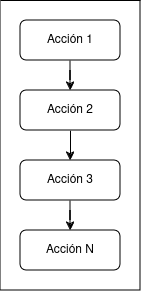
\includegraphics[width=0.25\textwidth]{images/secuencia.png}
    \caption{Ejemplo de secuencia}
    \centering Fuente: Elaboración propia
    \label{fig:acciones}
  \end{figure}

  \item \textbf{Selección} \\
  La estructura de selección, también conocida como toma de decisiones, permite que un programa ejecute diferentes instrucciones dependiendo de si se cumple una determinada condición lógica. Las estructuras de selección más comunes son las declaraciones ``if`` y ``else'', que permiten al programa elegir entre dos o más caminos basados en condiciones específicas. Por ejemplo, un programa puede decidir qué acción tomar según el valor de una variable o el resultado de una operación. La estructura de selección es fundamental para escribir programas que respondan de manera diferente a diferentes situaciones o entradas.
  \begin{figure}[h]
    \centering
    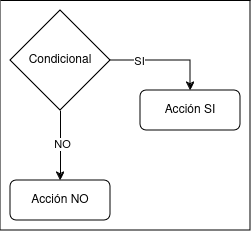
\includegraphics[width=0.4\textwidth]{images/seleccion.png}
    \caption{Ejemplo de selección}
    \centering Fuente: Elaboración propia
    \label{fig:seleccion}
  \end{figure}
  \newline

  \item \textbf{Iteración} \\
  La estructura de iteración, también conocida como bucle, permite que un bloque de código se repita varias veces hasta que se cumpla una determinada condición de salida. Esto permite la ejecución repetida de un conjunto de instrucciones sin tener que escribir el mismo código una y otra vez. Los bucles son esenciales para realizar tareas repetitivas de manera eficiente, como procesar grandes cantidades de datos o realizar operaciones en una lista o matriz. Las estructuras de bucle más comunes son "for", "while" y "do-while", cada una con sus propias características y casos de uso específicos. La estructura de iteración es crucial para la automatización de tareas y la optimización del rendimiento en programas informáticos.
  \begin{figure}[h]
    \centering
    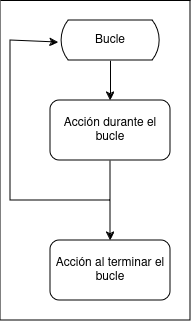
\includegraphics[width=0.3\textwidth]{images/iteracion.png}
    \caption{Ejemplo de iteración}
    \centering Fuente: Elaboración propia
    \label{fig:iteracion}
  \end{figure}
  \newline
\end{itemize}

\subsection{Ventajas y desventajas de la programación estructurada}
La programación estructurada es un paradigma de programación que promueve la mejora de la claridad, calidad y desarrollo de programas informáticos. A continuación, se detallan las ventajas y desventajas de este enfoque:

\subsubsection{Ventajas de la programación estructurada}
\begin{itemize}
  \item \textbf{Claridad y mantenimiento} \\
  La programación estructurada mejora significativamente la claridad del código. Al usar estructuras de control como bucles, condicionales y subrutinas, el flujo del programa se vuelve más comprensible y predecible. Esto facilita tanto la escritura como la lectura del código, lo cual es esencial para el mantenimiento a largo plazo y la colaboración entre múltiples desarrolladores. Programas claros y bien documentados son más fáciles de actualizar y depurar (Dijkstra, 1968).

  \item \textbf{Reutilización y modularidad} \\
  Este enfoque permite la creación de módulos o subrutinas reutilizables. La modularidad facilita la reutilización del código en diferentes partes del programa o incluso en diferentes proyectos. Esto no solo reduce el tiempo de desarrollo, sino que también disminuye la probabilidad de errores, ya que el código reutilizado ha sido previamente probado y validado. (Dijkstra, 1968).

  \item \textbf{Detección y corrección de errores} \\
  La estructura ordenada y lógica de los programas estructurados facilita la localización de errores. Los programas divididos en módulos independientes permiten identificar y corregir errores de manera más eficiente. Cada módulo puede ser probado individualmente antes de integrarlo en el programa completo, lo que simplifica la identificación de errores y su resolución. (Dijkstra, 1968).
\end{itemize}

\begin{table}[!h]
  \begin{center}
    \begin{tabularx}{0.8\textwidth}{|X|X|}
      \hline
      \textbf{Ventajas} & \textbf{Desventajas} \\
      \hline
      Claridad y mantenimiento & Rigidez y complejidad en programas grandes \\
      \hline
      Reutilización y modularidad & Rendimiento y flexibilidad limitados \\
      \hline
      Detección y corrección de errores & Curva de aprendizaje \\
      \hline
    \end{tabularx}
  \end{center}
  \caption{Comparativa de ventajas y desventajas}
  \centering Fuente: Elaboración propia
  \label{tab:ventajas}
\end{table}

La programación estructurada, con su enfoque en la claridad, la modularidad y la detección eficiente de errores, ofrece numerosas ventajas para el desarrollo de software. Sin embargo, también presenta desafíos, especialmente en proyectos grandes y complejos, donde la rigidez y las limitaciones de rendimiento pueden convertirse en problemas significativos.

\subsubsection{Desventajas de la programación estructurada}

\begin{itemize}
  \item \textbf{Rigidez y complejidad en programas grandes} \\
  A medida que los programas se vuelven más grandes y complejos, la programación estructurada puede volverse rígida. Mantener una estructura estrictamente organizada puede ser desafiante, y la adición de nuevas funcionalidades puede requerir modificaciones significativas en múltiples partes del código. Esto puede llevar a una mayor complejidad en el mantenimiento y evolución del software. (Dijkstra, 1968)
  \item \textbf{Rendimiento y flexibilidad limitados} \\
  La programación estructurada puede no ser la mejor opción para aplicaciones que requieren un rendimiento muy alto o una gran flexibilidad. Algunas optimizaciones de rendimiento, como la programación concurrente o la manipulación de bajo nivel de recursos, pueden ser más difíciles de implementar de manera eficiente dentro del marco estructurado. Esto puede limitar el rendimiento del programa en situaciones críticas. (Dijkstra, 1968).
  \item \textbf{Curva de aprendizaje} \\
  Aunque la programación estructurada promueve buenas prácticas, puede tener una curva de aprendizaje pronunciada para los principiantes. Comprender y aplicar correctamente las estructuras de control, la modularidad y la separación de funciones puede ser un desafío para los nuevos programadores. Esto requiere una educación y formación adecuada para asegurar que los desarrolladores puedan aprovechar plenamente las ventajas de este paradigma. (Dijkstra, 1968).
\end{itemize}

\section{Compiladores e intérpretes}
\subsection{Definición y funciones de un compilador}
Un compilador, en el contexto de la informática, es una herramienta esencial que despliega un conjunto de funciones clave para traducir programas escritos en lenguajes de alto nivel a un formato ejecutable por una computadora. Sus funciones principales se pueden desglosar en varias etapas:

\begin{itemize}
  \item \textbf{Análisis léxico} \\
  En la primera fase, el compilador realiza un análisis léxico, escaneando el código fuente para identificar y clasificar elementos léxicos como palabras clave, operadores y variables. Este proceso implica la creación de tokens que representan unidades léxicas básicas, proporcionando la base para etapas posteriores (Cooper \& Torczon, 2012).
  \item \textbf{Análisis sintáctico} \\
  La fase de análisis sintáctico sigue al análisis léxico y se centra en la estructura gramatical del código fuente. Aquí, se verifica que las secuencias de tokens sigan la gramática del lenguaje de programación. El resultado es un árbol sintáctico que representa la estructura jerárquica del programa, facilitando la comprensión y manipulación del código (Anderson, 2010).
  \item \textbf{Análisis semántico} \\
  El análisis semántico se encarga de verificar la coherencia y consistencia del código fuente en términos de significado y contexto. Se asegura de que las operaciones y expresiones sean válidas y tengan sentido dentro del lenguaje de programación. Este proceso es fundamental para detectar errores y garantizar la integridad del programa (Anderson, 2010).
  \item \textbf{Generación de código intermedio} \\
  Después del análisis sintáctico, se genera un código intermedio que sirve como representación abstracta del programa. Este código intermedio facilita la optimización del programa antes de generar el código objeto final. Durante esta fase, el compilador busca oportunidades para mejorar la eficiencia y la legibilidad del código (Cooper \& Torczon, 2012).
  \item \textbf{Optimización de código} \\
  La optimización de código es una etapa crucial en la que el compilador aplica diversas técnicas para mejorar el rendimiento del programa resultante. Esto incluye la eliminación de código redundante, la reorganización de instrucciones para minimizar el uso de recursos y la aplicación de estrategias para reducir la complejidad del programa (Cooper \& Torczon, 2012).
  \item \textbf{Generación de código objeto} \\
  La última fase implica la traducción del código intermedio optimizado a código objeto específico para la plataforma de destino. Este código objeto es un conjunto de instrucciones de bajo nivel comprensibles por la arquitectura del hardware de la computadora. El resultado final es un programa ejecutable que puede ser lanzado en la máquina objetivo (Cooper \& Torczon, 2012).
\end{itemize}

En conjunto, estas funciones convierten al compilador en una pieza esencial del desarrollo de software, permitiendo que los programas escritos en lenguajes de alto nivel se ejecuten eficientemente en los sistemas informáticos.

\subsection{Definición y funciones de un intérprete}
A diferencia de un compilador, un intérprete es una herramienta de ejecución de programas que opera directamente sobre el código fuente, sin necesidad de generar un archivo ejecutable independiente. Sus funciones clave se centran en la interpretación dinámica y la ejecución del código en tiempo real. Aquí se describen las principales funciones de un intérprete:

\begin{itemize}
  \item \textbf{Análisis léxico y sintáctico en tiempo real} \\
  Un intérprete analiza el código fuente durante la ejecución, realizando el análisis léxico y sintáctico en tiempo real. En lugar de realizar una fase de análisis previa, como en el caso de un compilador, el intérprete interpreta y ejecuta las instrucciones directamente del código fuente, lo que facilita una respuesta inmediata a posibles errores o cambios en el programa (Jeffery, 2021).
  \item \textbf{Interpretación directa} \\
  El intérprete ejecuta las instrucciones del código fuente sin generar un código intermedio o un archivo ejecutable independiente. Cada vez que se ejecuta el programa, el intérprete interpreta y ejecuta las instrucciones directamente, eliminando la necesidad de una fase de compilación previa (Jeffery, 2021).
  \item \textbf{Menor optimización} \\
  A diferencia de un compilador, un intérprete generalmente realiza menos optimizaciones exhaustivas. La optimización se realiza en tiempo real durante la ejecución, lo que puede resultar en un rendimiento ligeramente inferior en comparación con un programa compilado (Jeffery, 2021).
  \item \textbf{Adaptabilidad} \\
  La principal ventaja de un intérprete radica en su adaptabilidad. Los cambios en el código fuente pueden reflejarse de inmediato durante la ejecución sin la necesidad de pasar por una fase de compilación. Esto facilita el desarrollo iterativo y la depuración rápida, ya que los programadores pueden ver los resultados casi instantáneamente (Jeffery, 2021).
\end{itemize}

En resumen, un intérprete es una herramienta dinámica que analiza y ejecuta el código fuente en tiempo real, ofreciendo adaptabilidad y facilitando el desarrollo ágil. Aunque puede tener un rendimiento ligeramente inferior en comparación con un código compilado, su capacidad para reflejar cambios de manera inmediata lo hace valioso en contextos de desarrollo rápido y pruebas iterativas.

\subsection{Diferencias clave: compilador vs. intérprete}
Las diferencias entre un compilador y un intérprete residen principalmente en su enfoque hacia la generación de código, la eficiencia resultante y la portabilidad de los programas. Estas diferencias sustanciales proporcionan perspectivas esenciales sobre cómo cada uno maneja la ejecución de programas y las consecuencias que estas elecciones conllevan en el ámbito del desarrollo de software.

\begin{itemize}
  \item \textbf{Generación de código} \\
  Un compilador, en su esencia, lleva a cabo la generación de código como una etapa previa al tiempo de ejecución. Este proceso implica la conversión del código fuente de alto nivel en un formato ejecutable o en un código intermedio que posteriormente se traduce a instrucciones específicas para la máquina objetivo. Por el contrario, un intérprete opera directamente sobre el código fuente en tiempo real, analizando y ejecutando las instrucciones de manera secuencial sin la necesidad de generar un archivo ejecutable independiente (Alfonseca Moreno et al., 2006).
  \item \textbf{Eficiencia} \\
  La eficiencia se erige como una distinción marcada entre compiladores e intérpretes. Los programas compilados, debido a las optimizaciones exhaustivas realizadas durante la fase de compilación, tienden a exhibir un rendimiento superior. El código resultante está meticulosamente adaptado a la arquitectura de la máquina objetivo. Por otro lado, los intérpretes pueden experimentar un rendimiento ligeramente inferior ya que ejecutan directamente el código fuente, incurriendo en el costo de interpretación durante la ejecución (Alfonseca Moreno et al., 2006).
  \item \textbf{Portabilidad} \\
  En cuanto a la portabilidad, los intérpretes generalmente presentan una ventaja considerable. Dado que el código fuente puede ejecutarse directamente, los programas interpretados son inherentemente más portátiles entre diferentes plataformas. Contrariamente, los compiladores generan código específico para la plataforma de destino, lo que puede limitar la portabilidad del código compilado entre diversas arquitecturas o sistemas operativos. No obstante, con la presencia de compiladores cruzados y máquinas virtuales, esta limitación se ve mitigada en algunos contextos (Alfonseca Moreno et al., 2006).
\end{itemize}

Estas diferencias fundamentales arrojan luz sobre las consideraciones cruciales que los desarrolladores deben tener en cuenta al elegir entre un compilador y un intérprete según las necesidades y requisitos particulares de un proyecto. Mientras que los compiladores se destacan por ofrecer un rendimiento optimizado, los intérpretes se distinguen por su adaptabilidad y facilidad de uso, especialmente en entornos de desarrollo ágil y pruebas iterativas.

\section{Estructura de un intérprete}
Cuando se aborda la construcción de un intérprete, suele ser beneficioso adoptar una Representación Interna (RI) del lenguaje fuente a analizar. En este enfoque, la organización interna del intérprete se divide en módulos distintos:

\subsection{Traductor a representación interna}
Este módulo toma como entrada el código del programa en el Lenguaje Fuente. Analiza dicho código y lo transforma en la representación interna correspondiente al programa. (Labra Gayo et al., 2003).

\subsection{Representación interna (P/RI)}
La representación interna debe ser coherente con el programa original. Los árboles sintácticos son comúnmente utilizados como representación interna, y en casos donde sea viable, también se pueden emplear estructuras de pila para lograr una mayor eficiencia. (Labra Gayo et al., 2003).

\subsection{Tabla de símbolos}
Durante el proceso de traducción, se crea una tabla que almacena información relativa a los símbolos presentes en el código. La información almacenada puede incluir etiquetas para instrucciones de salto, detalles sobre identificadores (nombre, tipo, línea de aparición, etc.) u otra información necesaria en la etapa de evaluación. (Labra Gayo et al., 2003).

\begin{table}[!h]
  \begin{center}
    \begin{tabularx}{0.8\textwidth}{|X|X|}
      \hline
      \textbf{Operador} & \textbf{Significado} \\
      \hline
      $!$ & Negación \\
      \hline
      $+$ & Suma \\
      \hline
      $-$ & Resta \\
      \hline
      $*$ & Multiplicación \\
      \hline
      $/$ & División \\
      \hline
      $\%$ & Módulo \\
      \hline
      $<$ & Menor \\
      \hline
      $\leq$ & Menor igual \\
      \hline
      $>$ & Mayor \\
      \hline
      $\geq$ & Mayor igual \\
      \hline
      $!=$ & Diferente \\
      \hline
      $==$ & Igualdad \\
      \hline
      $\&\&$ & Conjunción lógica (Y) \\
      \hline
      $||$ & Disyunción lógica (O) \\
      \hline
    \end{tabularx}
  \end{center}
  \caption{Tabla de símbolos}
  \centering Fuente: (lu1tr0n, 2016)
  \label{tab:simbolos}
\end{table}

\subsection{Evaluador de representación interna}
Este módulo utiliza la representación interna generada y los datos de entrada para llevar a cabo las acciones necesarias y obtener los resultados esperados. Durante el proceso de evaluación, se deben contemplar posibles errores que puedan surgir (Labra Gayo et al., 2003).

\subsection{Tratamiento de errores}
Se gestiona el tratamiento de errores que podrían surgir durante el proceso de evaluación, como desbordamiento de la pila o divisiones por cero, entre otros (Labra Gayo et al., 2003).

Dependiendo de la complejidad del código a analizar, el intérprete puede incluir módulos similares a los de un compilador tradicional, como el análisis léxico, sintáctico y semántico. Durante la evaluación, el intérprete interactúa con los recursos del sistema, como la memoria y los discos. En muchos sistemas interpretados, se libera al programador de la gestión explícita de la memoria mediante técnicas de recolección de basura (Labra Gayo et al., 2003).

En el proceso de evaluar la representación interna, existen dos métodos fundamentales: la interpretación iterativa y la interpretación recursiva. Estos métodos definen cómo se llevarán a cabo las operaciones sobre la representación interna para obtener los resultados finales (Labra Gayo et al., 2003).

\section{Diseño de lenguajes de programación}
\subsection{Componentes principales del diseño}
El diseño de lenguajes de programación implica varios componentes fundamentales que aseguran su funcionalidad y eficiencia. Estos componentes incluyen el análisis léxico, que convierte el código fuente en una secuencia de tokens; el análisis sintáctico, que organiza estos tokens en una estructura jerárquica coherente; y el análisis semántico, que verifica la validez lógica de las estructuras sintácticas. Además, el diseño considera la implementación de un intérprete o compilador para ejecutar el código, la definición de la semántica y sintaxis del lenguaje, y la gestión de memoria y optimización del rendimiento. Estos elementos colaboran para crear un lenguaje de programación eficiente y funcional.

\subsubsection{Tokens y su manejo}
Los tokens son las unidades léxicas más pequeñas de un lenguaje de programación, y su manejo es una parte crucial del análisis léxico. Un token puede representar una palabra clave, un identificador, un literal (como un número o una cadena), un operador o un delimitador. El proceso de tokenización convierte una cadena de caracteres del código fuente en una secuencia de tokens que pueden ser procesados por el analizador sintáctico. Este proceso es fundamental para la correcta interpretación y compilación del código, ya que permite descomponer el texto en componentes manejables y significativos. (Jeffery, 2021).

El manejo de tokens implica definir claramente los diferentes tipos de tokens que el lenguaje soporta y cómo se deben identificar. En el diseño de lenguajes de programación, los tokens se categorizan típicamente en varias clases, como se muestra en la tabla siguiente:

\begin{table}
  \begin{center}
    \begin{tabularx}{0.8\textwidth}{|X|X|X|}
      \hline
      \textbf{Tipo de Token} & \textbf{Descripción} & \textbf{Ejemplo} \\
      \hline
      Palabra clave & Identifica las palabras reservadas del lenguaje & if, else, … \\
      \hline
      Identificador & Nombres de variables, funciones, etc. & variable, suma, … \\
      \hline
      Literal & Valores constantes & 123, “hola mundo”, … \\
      \hline
      Operador & Símbolos que representan operaciones & $+, -, *, … $\\
      \hline
      Delimitador & Símbolos que separan las estructuras del lenguaje & $;, \{\}, (), …$ \\
      \hline
    \end{tabularx}
  \end{center}
  \caption{Ejemplo de tokens}
  \centering Fuente: Elaboración propia
  \label{tab:tokens}
\end{table}

La importancia del manejo adecuado de tokens no puede subestimarse, ya que afecta directamente a la precisión del análisis sintáctico y la ejecución del código. Un sistema de tokenización bien diseñado puede detectar errores léxicos tempranos y proporcionar mensajes de error significativos, mejorando así la experiencia del desarrollador y la confiabilidad del software.

Un sistema de tokenización bien diseñado no solo organiza el código en componentes manejables, sino que también juega un papel crucial en la detección temprana de errores léxicos. Al identificar errores en esta etapa inicial del proceso de compilación, se evita que errores menores escalen a problemas más complejos en fases posteriores, lo que facilita su corrección y mejora la calidad del software. (Jeffery, 2021).

A continuación, se presenta un diagrama de flujo básico que ilustra el proceso de tokenización:
\begin{figure}[!h]
  \centering
  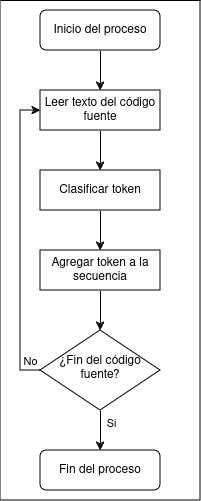
\includegraphics[width=0.27\textwidth]{images/tokenizacion.png}
  \caption{Proceso de tokenización}
  \centering Fuente: Elaboración propia
  \label{fig:tokenizacion}
\end{figure}

En el diagrama, el flujo comienza con la entrada del código fuente, que es analizado carácter por carácter para identificar y categorizar los diferentes tokens. Este flujo asegura que cada componente del código sea correctamente identificado y clasificado, lo que es crucial para las etapas posteriores de análisis sintáctico y semántico.

\subsubsection{Estructuras léxicas}
Las estructuras léxicas son las reglas y patrones que definen cómo se reconocen y agrupan las secuencias de caracteres en el código fuente para formar los tokens. Estas estructuras incluyen la definición de patrones para palabras clave, identificadores, operadores, símbolos especiales, constantes numéricas y constantes de caracteres. El analizador léxico utiliza estas reglas para convertir el texto del código fuente en una secuencia de tokens que el analizador sintáctico pueda procesar.

\begin{itemize}
  \item \textbf{Patrón} \\
  Un patrón es una regla que describe la secuencia de caracteres que puede formar un determinado token. Por ejemplo, el patrón para un identificador podría ser una letra seguida de cualquier combinación de letras y dígitos. Los patrones se definen utilizando expresiones regulares o gramáticas formales, y son fundamentales para la correcta identificación de los tokens. (Jeffery, 2021).
  \item \textbf{Lexema} \\
  Un lexema es una cadena de caracteres del código fuente que coincide con un patrón específico. Por ejemplo, en la expresión x = 10;, los lexemas incluyen x, =, 10, y ;. Cada lexema se asocia con un token que describe su tipo y, en algunos casos, su valor. (Jeffery, 2021).
  \item \textbf{Componente léxico} \\
  Un componente léxico, o token, es el resultado de la agrupación de un lexema según su patrón correspondiente. Un componente léxico puede tener uno o varios lexemas asociados. Por ejemplo, las palabras clave como if y while tienen un único lexema, mientras que los identificadores y números pueden tener infinitos lexemas diferentes. (Jeffery, 2021).
\end{itemize}

En la siguiente tabla se muestran algunos ejemplos:

\begin{table}[!h]
  \begin{center}
    \begin{tabularx}{0.8\textwidth}{|X|X|X|}
      \hline
      \textbf{Tipo de Token} & \textbf{Patrón} & \textbf{Ejemplo} \\
      \hline
      Palabra clave & if, while, … & if, while, … \\
      \hline
      Identificador & $[a-zA-Z\_] [a-zA-Z\_0-9]*$ & variable, x, … \\
      \hline
      Operador & $\backslash +, ==, -, =, …$ & $+, ==, …$ \\
      \hline
      Constante numérica & $[0-9]+(\backslash .[0-9]+)?$ & $42, 3.14, …$ \\
      \hline
      Constante de caracteres & $``.", [\land "]*$ & 'a', "hola", … \\
      \hline
    \end{tabularx}
  \end{center}
  \caption{Ejemplo de patrones y lexemas}
  \centering Fuente: Elaboración propia
  \label{tab:patrones}
\end{table}

En resumen, las estructuras léxicas son las bases que permiten al analizador léxico reconocer y clasificar cada elemento del código fuente en su correspondiente token, facilitando el análisis y procesamiento del código en las etapas posteriores de compilación o interpretación.

\subsubsection{Estructuras sintácticas}
Las estructuras sintácticas definen las reglas que gobiernan cómo se combinan los tokens para formar sentencias y programas válidos. Estas reglas se especifican mediante una gramática formal, que puede ser usada por un analizador sintáctico para construir un árbol de análisis sintáctico (AST) del código fuente.

\paragraph{Análisis sintáctico}

Un analizador sintáctico constituye una componente esencial en el desarrollo de un sistema de interpretación de código. Su función principal radica en convertir la entrada proporcionada en una estructura jerárquica más significativa, comúnmente representada mediante un árbol de derivación (Ortín Soler et al., 2004).

Este proceso sintáctico se encarga de transformar el texto de entrada en otras estructuras, como árboles, que facilitan análisis subsiguientes y capturan la jerarquía subyacente en la entrada. Un analizador léxico previo se encarga de generar tokens a partir de la secuencia de caracteres de entrada. Estos tokens, a su vez, son procesados por el analizador sintáctico para construir la estructura de datos deseada, como por ejemplo un árbol de análisis o árboles de sintaxis abstracta.

No solo limitado al ámbito de compiladores, el análisis sintáctico encuentra aplicación en la etapa inicial del procesamiento de frases en lenguaje natural. En este contexto, se utiliza para generar diagramas en idiomas que hacen uso de la flexión gramatical, como los idiomas romances o el latín. Los analizadores sintácticos son especialmente eficaces en la interpretación de lenguajes que cumplen con la condición de ser libres de contexto (Ortín Soler et al., 2004).

Es relevante destacar que existe una fundamentación formal que establece que los lenguajes libres de contexto son aquellos que pueden ser reconocidos por un autómata de pila. De esta manera, todo analizador sintáctico capaz de reconocer un lenguaje libre de contexto es equivalente en capacidad computacional a un autómata de pila. Este hecho proporciona un marco teórico sólido para comprender la potencia y alcance de los analizadores sintácticos en el ámbito de la interpretación de lenguajes. (Ortín Soler et al., 2004).

\paragraph{Gramática formal}

Es un conjunto de reglas que definen la sintaxis de un lenguaje de programación. Estas reglas especifican cómo se pueden combinar los elementos básicos del lenguaje, conocidos como tokens, para formar estructuras sintácticas válidas, como expresiones, declaraciones y programas completos. Las gramáticas formales son esenciales en el diseño de lenguajes de programación y en la construcción de analizadores sintácticos. (Ortín Soler et al., 2004).

\subparagraph{Componentes de una gramática formal}

Una gramática formal se compone de cuatro componentes principales:

\begin{itemize}
  \item \textbf{Conjunto de símbolos terminales (T)} \\
  Son los elementos básicos del lenguaje, los tokens, que no se pueden descomponer más. Estos incluyen palabras clave (como if, while), operadores (como $+, *$), y delimitadores (como $;, (, )$).
  \item \textbf{Conjunto de símbolos no terminales (N)} \\
  Son categorías sintácticas que pueden ser descompuestas en una secuencia de símbolos terminales y no terminales. Ejemplos de símbolos no terminales son <expresión>, <declaración>, y <bloque>.
  \item \textbf{Conjunto de reglas de producción (P)} \\
  Son las reglas que definen cómo los símbolos no terminales pueden ser expandidos en secuencias de símbolos terminales y no terminales. Cada regla de producción tiene la forma $A \rightarrow \alpha$, donde $A$ es un símbolo no terminal y $\alpha$ es una secuencia de símbolos terminales y/o no terminales. Por ejemplo, una regla de producción podría ser <expresión> $\rightarrow$ <términod> $'+'$ <término>.
\end{itemize}

\paragraph{Árbol de análisis sintáctico (AST)}

El árbol de análisis sintáctico, conocido como AST (Abstract Syntax Tree), es una representación jerárquica de la estructura sintáctica de un programa. A diferencia de un árbol de derivación, el AST omite detalles de la gramática que no son esenciales para la semántica del programa y se enfoca en capturar las relaciones estructurales y lógicas entre las diferentes partes del código. (Jeffery, 2021).

\subparagraph{Características del AST}

\begin{itemize}
  \item \textbf{Nodos} \\
  Cada nodo en el AST representa una construcción sintáctica significativa del lenguaje de programación, como expresiones, declaraciones, y bloques de código.
  \item \textbf{Hijos de nodos} \\
  Los hijos de un nodo representan los componentes constituyentes de esa construcción sintáctica. Por ejemplo, un nodo que representa una expresión de suma tendrá dos hijos: uno para cada operando.
  \item \textbf{Eliminación de información irrelevante} \\
  El AST elimina información redundante como delimitadores (paréntesis, punto y coma) que son necesarios en la gramática, pero no son necesarios para entender la estructura lógica del programa.
\end{itemize}

\subparagraph{Construcción del AST}
La construcción del Árbol de Análisis Sintáctico (AST) se lleva a cabo durante la fase de análisis sintáctico del proceso de compilación o interpretación. Este proceso comienza después de que el analizador léxico ha convertido el código fuente en una secuencia de tokens. El analizador sintáctico utiliza una gramática formal para analizar esta secuencia de tokens y generar el AST. Durante este análisis, el parser (analizador sintáctico) sigue las reglas de la gramática para identificar construcciones sintácticas válidas y crear nodos correspondientes en el árbol. Cada regla de producción de la gramática se traduce en una estructura jerárquica en el AST, donde los nodos representan las construcciones sintácticas y sus relaciones lógicas.

El proceso de construcción del AST implica varios pasos. Primero, el analizador sintáctico lee los tokens y aplica las reglas de producción de la gramática para agruparlos en estructuras mayores. Por ejemplo, una regla de producción podría especificar que una expresión aritmética se compone de un término seguido de un operador y otro término. A medida que el parser reconoce esta estructura, crea un nodo para el operador y agrega nodos hijos para los términos. Este proceso continúa recursivamente, con el parser construyendo subárboles para subexpresiones y combinándolos en estructuras más grandes hasta que todo el código fuente se ha procesado y se ha construido un AST completo. Esta estructura jerárquica es esencial para las etapas posteriores de compilación, como el análisis semántico y la generación de código, ya que proporciona una representación clara y manipulable de la lógica del programa. (Jeffery, 2021).

El uso del AST ofrece varias ventajas en el procesamiento del código fuente:

\begin{itemize}
  \item \textbf{Claridad y simplicidad} \\
  Al omitir detalles innecesarios de la gramática, el AST proporciona una representación más clara y manejable de la estructura del programa.
  \item \textbf{Facilita el análisis semántico} \\
  El AST es una base excelente para realizar el análisis semántico, donde se verifican tipos de datos, alcances de variables, y otras propiedades semánticas del código.
  \item \textbf{Optimización del código} \\
  Las optimizaciones del código son más fáciles de aplicar en el AST, ya que proporciona una visión estructural del programa que puede ser manipulada para mejorar el rendimiento.
  \item \textbf{Generación de código} \\
  La generación de código intermedio o código máquina a partir del AST es más directa, ya que el árbol captura las relaciones semánticas necesarias para traducir el programa a un lenguaje de bajo nivel.
\end{itemize}

\begin{figure}[!h]
  \centering
  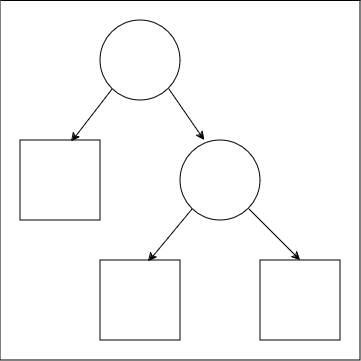
\includegraphics[width=0.5\textwidth]{images/ast.png}
  \caption{Ejemplo de Árbol de Análisis Sintáctico (AST)}
  \centering Fuente: Elaboración propia
  \label{fig:ast}
\end{figure}

\paragraph{Ejemplo de una gramática formal}
Consideremos un pequeño subconjunto de un lenguaje de programación que incluye expresiones aritméticas y asignaciones. A continuación, se muestra una posible gramática formal para este subconjunto:

\begin{itemize}
  \item \textbf{Símbolos terminales (T)} \\
  $id$ (identificador), $num$ (número), $+$ (suma), $-$ (resta), $*$ (multiplicación), $/$ (división), $=$ (asignación), $(, )$ (paréntesis).
  \item \textbf{Símbolos no terminales (N)} \\
  <programa>, <sentencia>, <expresión>, <término>, <factor>.
  \item \textbf{Símbolo inicial (S)} \\
  <programa>.
  \item \textbf{Reglas de producción (P)} \\
  <programa> $\rightarrow$ <sentencia> \\
  <sentencia> $\rightarrow$ $id$ `$=$' <expresión> \\
  <expresión> $\rightarrow$ <termino> \space $|$ <expresión> '$+$' <término> \\
  <término> $\rightarrow$ <factor> \space $|$ <término> '$*$' <factor> \\
  <factor> $\rightarrow$ $id$ \space $|$ $num$ \space $|$ '(' <expresión> ')'
\end{itemize}

Utilizando la gramática anterior, podemos derivar la sentencia $x = 3 + 5 * (2 + 1)$ de la siguiente manera:
\begin{equation*}
  \begin{split}
    <pr&ograma> \\
    <se&ntencia> \\
    id & = <expresi\acute{o}n> \\
    id & = <t\acute{e}rmino> + <t\acute{e}rmino> \\
    id & = <factor> + <t\acute{e}rmino> \\
    id & = num + <t\acute{e}rmino> \\
    id & = 3 + <t\acute{e}rmino> \\
    id & = 3 + <factor> * <t\acute{e}rmino> \\
    id & = 3 + num * <t\acute{e}rmino> \\
    id & = 3 + 5 * ( <expresi\acute{o}n> ) \\
    id & = 3 + 5 * ( <factor> + <factor> ) \\
    id & = 3 + 5 * ( num + num) \\
    id & = 3 + 5 * ( 2 + 1 )
  \end{split}
\end{equation*}

El Árbol de Sintaxis Abstracta (AST) es fundamental en el análisis y procesamiento de programas, proporcionando una representación clara y eficiente del código fuente. Facilita el análisis semántico al permitir verificaciones detalladas de la lógica y las reglas del lenguaje, y contribuye a la optimización al ofrecer una estructura sobre la cual se pueden aplicar transformaciones para mejorar la eficiencia. Además, el AST guía la generación de código al traducir la representación abstracta en instrucciones ejecutables, asegurando que el software sea tanto funcional como optimizado.

El AST para esta expresión sería:

\begin{figure}[!h]
  \centering
  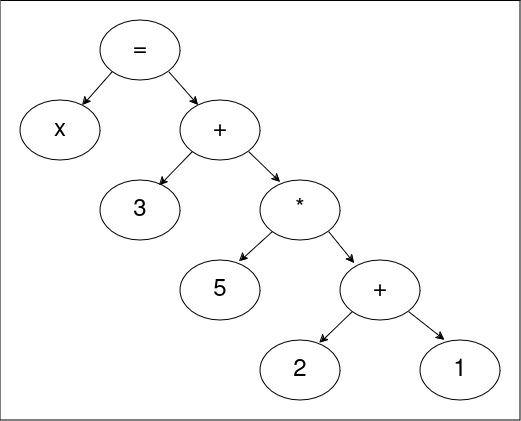
\includegraphics[width=0.6\textwidth]{images/ast_ejemplo.png}
  \caption{Árbol AST del ejemplo}
  \centering Fuente: Elaboración propia
  \label{fig:ast_ejemplo}
\end{figure}

Este diagrama ilustra cómo una expresión aritmética se descompone en sus componentes básicos y se organiza en una estructura jerárquica. Cada nodo del árbol representa una operación o un valor, mostrando claramente la relación entre los diferentes elementos de la expresión.

\subsubsection{Análisis semántico}
Es una fase crítica en la implementación de un intérprete, enfocada en verificar la lógica del código fuente después de que este ha pasado por el análisis sintáctico. Durante esta etapa, se comprueba que las construcciones del programa tengan sentido dentro del contexto del lenguaje de programación. El análisis semántico se encarga de validar aspectos como la compatibilidad de tipos, la existencia y el alcance de variables, y la correcta invocación de funciones y procedimientos. Por ejemplo, si una variable es utilizada antes de ser declarada o si se intenta asignar un valor de tipo entero a una variable de tipo cadena, estos errores deben ser detectados en esta fase.

El proceso de análisis semántico involucra varias comprobaciones detalladas. Primero, la “verificación de tipos” asegura que las operaciones entre variables y constantes sean compatibles, lo cual evita errores como sumar un número con una cadena de texto. Segundo, el “chequeo de alcances y contextos” confirma que las variables y funciones sean accesibles en los lugares correctos del programa. Esto es particularmente importante en lenguajes que soportan estructuras de alcance anidado o variables locales y globales. Finalmente, la “validación de la correcta invocación de funciones” verifica que las funciones y procedimientos sean llamados con los argumentos correctos en términos de número y tipo. (Jeffery, 2021).

A continuación, se presenta una tabla que resume algunos de los errores semánticos comunes y cómo son gestionados en el análisis semántico:
\begin{table}[!h]
  \begin{center}
    \begin{tabularx}{0.85\textwidth}{|X|X|X|X|}
      \hline
      \textbf{Tipo de Error Semántico} & \textbf{Descripción} & \textbf{Ejemplo} & \textbf{Gestión del Error} \\
      \hline
      Incompatibilidad de Tipos & Operaciones realizadas entre tipos no compatibles & int x = "cadena"; & Reporte de error y terminación del análisis \\
      \hline
      Uso de Variables no Declaradas & Uso de variables que no han sido previamente declaradas & y = 5; (sin declarar y) & Advertencia o error según la política del lenguaje \\
      \hline
      Alcance Incorrecto de Variables & Acceso a variables fuera de su ámbito de declaración & print(x); fuera del bloque & Reporte de error indicando el alcance inválido \\
      \hline
      Invocación Incorrecta de Funciones & Llamadas a funciones con argumentos erróneos en tipo o número & func(1, ``cadena''); & Verificación de parámetros y reporte de inconsistencias \\
      \hline
    \end{tabularx}
  \end{center}
  \caption{Ejemplo de errores semánticos}
  \centering Fuente: Elaboración propia
  \label{tab:errores_semanticos}
\end{table}

\newpage
\subsubsection{Generación de código intermedio}
Es una fase que sigue al análisis semántico y precede a la ejecución del código. En esta etapa, el código fuente se transforma en una representación abstracta que no está directamente en lenguaje máquina, pero que es más fácil de manipular y optimizar. Este código intermedio sirve como un puente entre el código de alto nivel y la ejecución final, permitiendo optimizaciones y análisis adicionales que mejoran la eficiencia y la portabilidad del intérprete.

El código intermedio suele estar representado en una forma que conserva la estructura lógica del programa pero con una sintaxis simplificada y estandarizada. Algunas de las formas comunes de código intermedio incluyen el “código de tres direcciones y el lenguaje intermedio basado en registros”. Estas representaciones permiten la implementación de optimizaciones como la eliminación de código muerto, la fusión de bloques básicos, y la reducción de redundancias, mejorando así la eficiencia del intérprete. (Jeffery, 2021).

Un ejemplo sencillo de código intermedio puede ser la conversión de una expresión aritmética compleja en una serie de instrucciones más simples y directas. Consideremos la expresión a = b + c * d;. En código intermedio, esto podría representarse como:
\begin{equation*}
  \begin{split}
    t1 & = c * d; \\
    t2 & = b + t1; \\
    a & = t2;
  \end{split}
\end{equation*}

Estas instrucciones descomponen la expresión en pasos elementales, facilitando la posterior ejecución e interpretación. La claridad y simplicidad del código intermedio permiten una gestión más eficaz durante la fase de ejecución, así como una detección más temprana de posibles errores y optimizaciones.

\subsubsection{Evaluación y ejecución}
Es la etapa final en el proceso de implementación de un intérprete. En esta fase, el intérprete toma las instrucciones del código intermedio y las ejecuta una a una, llevando a cabo las operaciones definidas en el programa fuente. Durante esta etapa, se realizan varias tareas críticas, como la gestión de memoria para almacenar y recuperar datos, la manipulación de variables para asegurar que los valores se actualicen correctamente, y la llamada y retorno de funciones para controlar el flujo del programa. Además, se gestiona la entrada y salida de datos, permitiendo al programa interactuar con el usuario. Esta fase es esencial para la ejecución efectiva del código.

Durante la ejecución, es fundamental que el intérprete maneje adecuadamente los errores en tiempo de ejecución, como divisiones por cero, accesos a memoria no válidos, y otros errores lógicos que pueden surgir. La capacidad de detectar y manejar estos errores de manera eficaz es crucial para proporcionar retroalimentación útil al desarrollador y garantizar la robustez del intérprete. Además, el intérprete debe ser capaz de optimizar la ejecución en tiempo real, aplicando técnicas como la ejecución especulativa y la reordenación de instrucciones para mejorar el rendimiento sin comprometer la correcta ejecución del programa. (Jeffery, 2021).

El siguiente diagrama ilustra el flujo del proceso de implementación del intérprete, desde el análisis léxico hasta la evaluación y ejecución:
\begin{figure}[!h]
  \centering
  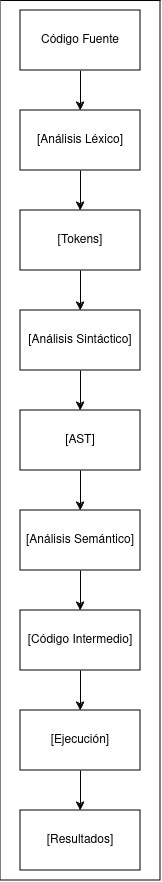
\includegraphics[width=0.2\textwidth]{images/flujo_interprete.png}
  \caption{Diagrama de la implementación del intérprete}
  \centering Fuente: Elaboración propia
  \label{fig:flujo_interprete}
\end{figure}
\newpage
Este enfoque estructurado asegura que cada fase del proceso de implementación esté bien definida y coordinada, garantizando la correcta ejecución del programa y la facilidad de mantenimiento y extensión del intérprete.

\section{Python}
Python es un lenguaje de programación de alto nivel que se utiliza para desarrollar aplicaciones de todo tipo. A diferencia de otros lenguajes como Java o .NET, se trata de un lenguaje interpretado, es decir, que no es necesario compilarlo para ejecutar las aplicaciones escritas en Python, sino que se ejecutan directamente por el ordenador utilizando un programa denominado interpretador, por lo que no es necesario “traducirlo” a lenguaje máquina (Santander Universidades, 2021).

La elección de Python como lenguaje de programación para el desarrollo de nuestro intérprete ofrece una serie de ventajas notables. En primer lugar, Python es reconocido por su facilidad de uso y su sintaxis legible, lo que simplifica el proceso de desarrollo y facilita la comprensión del código fuente. La naturaleza intuitiva de Python es especialmente beneficiosa para un proyecto como un intérprete, donde la claridad y la accesibilidad son fundamentales.

La amplia comunidad de desarrolladores de Python es otra ventaja significativa. Esta comunidad activa proporciona acceso a una extensa documentación y a una variedad de recursos en línea, lo que agiliza la resolución de problemas y la adopción de mejores prácticas en el desarrollo del intérprete.

La rica biblioteca estándar de Python es un recurso valioso para nuestro proyecto. Con una amplia gama de módulos y funciones predefinidos, podemos aprovechar estas herramientas para acelerar el desarrollo e implementar diversas funcionalidades en nuestro intérprete. La flexibilidad de Python también nos permite integrar bibliotecas y frameworks externos, lo que abre la puerta a una amplia variedad de herramientas adicionales para mejorar la funcionalidad y la eficiencia del intérprete.

Además, Python es conocido por su capacidad para abordar problemas de programación estructurada de manera clara y concisa. La sintaxis intuitiva del lenguaje facilita la implementación de estructuras de control y la gestión de datos, lo cual es esencial para nuestro intérprete de pseudocódigo en español, orientado a la programación estructurada. En resumen, la elección de Python ofrece una combinación de accesibilidad, recursos comunitarios y capacidad para abordar problemas de programación estructurada, haciendo que sea una opción sólida para el desarrollo de nuestro intérprete.

\section{Metodologías de trabajo}
Se adoptó la metodología Kanban como marco de trabajo. Kanban es una metodología ágil que se basa en la visualización del flujo de trabajo y la gestión de tareas de manera incremental. A diferencia de otros enfoques ágiles, Kanban no utiliza sprints fijos y permite una mayor flexibilidad en la gestión de tareas.

\subsection{Kanban}
La metodología Kanban nos ayudará a definir, gestionar y mejorar los servicios que entregan conocimiento, tales como servicios profesionales, trabajos o actividades en las que interviene la creatividad y el diseño tanto como productos de software como físicos. Su principio de la metodología es “Empieza por donde estés”, por lo cual nos permite realizar cambios de manera eficiente y enfocado en lo requerido por la organización, de igual manera ayuda a reducir la resistencia de evitar los cambios. (Garzas, 2011).

\begin{itemize}
  \item \textbf{Visualización del flujo de trabajo} \\
  La visualización del flujo de trabajo es un principio central en Kanban. Al adoptar esta práctica, se logra una representación clara y transparente de todas las tareas en el proceso de desarrollo, desde su concepción hasta su implementación final. La implementación de un tablero Kanban permite a todos los miembros del equipo, en este caso, al desarrollador individual, tener una visión instantánea de las tareas en curso y su estado actual. Cada tarea se representa como una tarjeta en el tablero, proporcionando información detallada sobre su progreso. La visualización facilita la identificación de posibles cuellos de botella, áreas de mejora y ayuda en la toma de decisiones informadas sobre la gestión de las tareas (Anderson, 2010).
  \begin{figure}[!h]
    \centering
    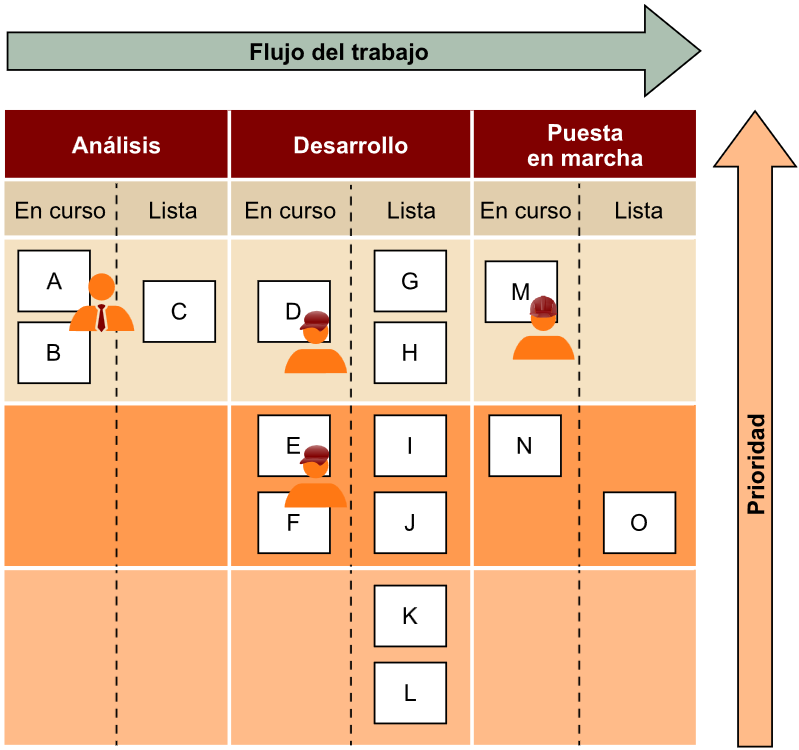
\includegraphics[width=0.55\textwidth]{images/kanban.png}
    \caption{Panel Kanban}
    \centering Fuente: (Bermejo, 2010)
    \label{fig:kanban}
  \end{figure}
  Se representa un panel compuesto por tres columnas que reflejan las diversas fases a través de las cuales una tarea debe fluir para su desarrollo: análisis, desarrollo y puesta en marcha. Cada fase se subdivide en dos estados, ``en curso'' y ``lista'', indicando si el equipo está actualmente trabajando en la tarea en esa fase o si la tarea ha sido completada y está lista para pasar a la siguiente fase. Esta división se destaca mediante una línea discontinua en cada fase, y sirve para identificar posibles atascos en el proceso de producción.
  
  El estado ``en curso'' implica que el equipo está activamente comprometido en la tarea durante esa fase, mientras que el estado ``lista'' significa que el trabajo en esa fase ha sido completado y la tarea está a la espera de ser tomada por el sistema para la siguiente fase. Esta subdivisión facilita la identificación de posibles cuellos de botella en el proceso de producción. Las filas pueden representar diferentes proyectos en los que la empresa está trabajando, pero es más común que indique la prioridad, donde las tareas en las filas superiores son las más prioritarias.
  
  La fase de puesta en marcha se divide en dos, con la fase de ``revisión de calidad''. En esta fase, cada tarea desarrollada es sometida a pruebas de calidad, que son realizadas por uno de los programadores utilizando criterios aprendidos del experto de sistemas.
  
  Se destaca que el límite de trabajo en progreso (WIP) para la fase de desarrollo se ha reducido de nueve a cinco. La reducción del límite de WIP se basa en las necesidades del proyecto y ayuda a evitar la acumulación excesiva de trabajo en una fase particular. Se menciona que aumentar el límite de WIP es una mala práctica. En la fase de revisión de calidad, todas las tareas deben ser finalizadas pasando por este proceso (Bermejo, 2010).

  \item \textbf{Limitación del trabajo en progreso} \\
  La imposición de límites al trabajo en progreso es esencial para mantener un flujo de trabajo constante y prevenir la sobrecarga del equipo de desarrollo. Establecer un límite en la cantidad de tareas permitidas en la columna "en curso" ayuda a evitar la multitarea excesiva y concentra la atención en completar tareas antes de comenzar nuevas. Esta limitación fomenta un enfoque más eficiente y eficaz en la resolución de problemas, ya que el desarrollador se centra en unas pocas tareas a la vez. Además, al limitar el trabajo en progreso, se reduce la probabilidad de que se generen cuellos de botella, lo que contribuye a un flujo de trabajo más suave y predecible (Anderson, 2010).

  \item \textbf{Gestión activa} \\
  La gestión activa en Kanban implica la revisión constante del tablero Kanban para identificar áreas de mejora y optimización del proceso de desarrollo. Esta práctica va más allá de la simple visualización y establecimiento de límites; implica una participación continua para evaluar y ajustar el flujo de trabajo. Mediante la gestión activa, se pueden realizar cambios en tiempo real para abordar problemas emergentes y mejorar la eficiencia del equipo de desarrollo. Esta mentalidad de mejora continua es fundamental para la evolución exitosa del proceso de desarrollo a lo largo del tiempo (Anderson, 2010).
\end{itemize}

\section{Licencia de uso}
La Licencia Pública General de GNU versión 3 (GPLv3) es una licencia de software libre desarrollada por la Free Software Foundation (FSF), diseñada para garantizar la libertad de los usuarios de software. Esta licencia establece una serie de permisos, limitaciones y condiciones que rigen el uso, modificación y distribución del software cubierto por ella. (GNU, 2021).

\subsection{Permisos}
\begin{itemize}
  \item \textbf{Uso del software} \\
  La GPLv3 otorga a cualquier persona el derecho de utilizar el software para cualquier propósito, sin restricciones.
  \item \textbf{Estudio y modificación} \\
  Los usuarios tienen la libertad de estudiar cómo funciona el software y adaptarlo a sus necesidades, incluyendo la modificación del código fuente.
  \item \textbf{Redistribución} \\
  La GPLv3 permite a los usuarios distribuir el software, tanto en su forma original como modificada, siempre y cuando se respeten los términos de la licencia.
  \item \textbf{Licencias derivadas} \\
  Los usuarios pueden crear y distribuir versiones modificadas del software bajo los términos de la GPLv3, garantizando que las mejoras estén disponibles para toda la comunidad.
\end{itemize}

\subsection{Limitaciones}
\begin{itemize}
  \item \textbf{Compatibilidad con otras licencias} \\
  La GPLv3 puede ser incompatible con ciertas licencias de software propietario, lo que podría limitar la combinación del software bajo licencia GPLv3 con otros programas.
  \item \textbf{Restricciones de patentes} \\
  La licencia incluye disposiciones para abordar el uso de patentes en relación con el software cubierto, asegurando que los usuarios estén protegidos de posibles reclamos de violación de patentes.
\end{itemize}

\subsection{Condiciones}
\begin{itemize}
  \item \textbf{Inclusión de la licencia} \\
  Cualquier redistribución del software debe incluir una copia de la GPLv3, así como los avisos de derechos de autor y responsabilidad correspondientes.
  \item \textbf{Disponibilidad del código fuente} \\
  El código fuente del software debe estar disponible o ser proporcionado bajo solicitud, sin costos adicionales más allá del costo razonable de la distribución.
  \item \textbf{Identificación de modificaciones} \\
  Las modificaciones realizadas al software deben ser claramente identificadas como tales, y los avisos de derechos de autor originales deben mantenerse intactos.
  \item \textbf{Compatibilidad con versiones anteriores} \\
  Las nuevas versiones del software pueden incluir términos adicionales o diferentes, pero estos no pueden anular los permisos otorgados por versiones anteriores de la GPLv3.
\end{itemize}

En resumen, la GPLv3 establece un marco legal que fomenta la libertad y la colaboración en el desarrollo de software, garantizando que el conocimiento y la tecnología estén disponibles para todos.

\section{Extensiones de VSCode}
\subsection{Visual Studio Code (VSCode)}
Visual Studio Code (VSCode), desarrollado por Microsoft, es un editor de código abierto y gratuito que ha ganado una gran popularidad en la comunidad de desarrollo de software. Destacado por su eficiencia y versatilidad, VSCode es compatible con múltiples sistemas operativos, incluyendo Windows, macOS y Linux. Su atractiva combinación de características, que incluyen soporte para múltiples lenguajes de programación, integración con Git y una amplia gama de extensiones, lo convierten en una herramienta imprescindible para desarrolladores de todos los niveles de experiencia. (García de Zúñiga, 2023).

En resumen, VSCode ofrece una experiencia de desarrollo ágil y potente, respaldada por una comunidad activa y una extensa biblioteca de extensiones, lo que lo convierte en una opción preferida para proyectos de software de cualquier tamaño.

\subsection{Funcionalidades y beneficios de las extensiones de VSCode}
Las extensiones de Visual Studio Code (VSCode) son complementos diseñados para mejorar y personalizar la experiencia del usuario dentro del editor. Estas extensiones pueden proporcionar desde funciones básicas como resaltado de sintaxis hasta características más avanzadas como herramientas de depuración específicas para ciertos lenguajes de programación. La versatilidad de las extensiones permite a los usuarios adaptar VSCode a sus necesidades específicas, lo que lo convierte en una herramienta altamente personalizable para una amplia gama de proyectos de desarrollo de software.

Una de las ventajas clave de las extensiones de VSCode es su capacidad para extender el soporte del editor a una amplia variedad de lenguajes de programación y tecnologías. Esto significa que los desarrolladores pueden trabajar en proyectos que utilicen diferentes tecnologías sin necesidad de cambiar de editor. Además, la comunidad activa de desarrolladores contribuye constantemente con nuevas extensiones y actualizaciones, lo que garantiza que VSCode siga siendo relevante y competitivo en el mundo del desarrollo de software (Nandwana, 2023).

En resumen, las extensiones de Visual Studio Code amplían las funcionalidades del editor y permiten a los usuarios adaptarlo a sus necesidades específicas. Desde mejorar el soporte para diferentes lenguajes hasta agregar nuevas características y herramientas, las extensiones juegan un papel fundamental en la versatilidad y la popularidad de VSCode entre los desarrolladores.

\section{Norma ISO 25010}
La norma ISO 25010, define un conjunto de requisitos y criterios de evaluación que permiten medir la calidad de un producto de software. (Ormeño, 2019). Estos requisitos se dividen en ocho atributos de calidad principales, que son:
\begin{itemize}
  \item \textbf{Funcionalidad} \\
  Capacidad de satisfacer las necesidades del usuario.
  \item \textbf{Fiabilidad} \\
  Capacidad de mantener su nivel de rendimiento en condiciones normales de uso.
  \item \textbf{Usabilidad} \\
  Capacidad de ser entendido, aprendido y utilizado por el usuario.
  \item \textbf{Eficiencia} \\
  Capacidad de utilizar los recursos de forma óptima para lograr los resultados deseados.
  \item \textbf{Mantenibilidad} \\
  Capacidad de ser modificado, corregido o mejorado de manera eficiente.
  \item \textbf{Portabilidad} \\
  Capacidad de ser transferido y utilizado en diferentes entornos.
  \item \textbf{Seguridad} \\
  Capacidad de proteger la información y los recursos del sistema.
  \item \textbf{Compatibilidad} \\
  Capacidad de interactuar con otros sistemas o componentes sin problemas.
\end{itemize}
\chapter{MARCO APLICATIVO}

Al ser un proyecto Open Source utilizar nombres en inglés en el desarrollo de software es preferible debido a su estandarización global en la industria. Esta práctica promueve la claridad, consistencia y accesibilidad del código, facilitando la colaboración internacional, la comprensión del código para desarrolladores futuros, y la búsqueda de recursos y documentación en línea. Además, favorece la reutilización del código en diferentes contextos y proyectos, mejorando la eficiencia y la calidad del desarrollo de software en general.

\section{Metodología de trabajo}
Las diferentes tareas se irán registrando en el tablero, a su vez, con el apoyo visual que brinda, facilita el saber en qué punto se encuentra cada actividad. Al ser un proyecto pensado para ser distribuido como Open Source, el tablero también sirve para crear nuevas Issues que cualquier contribuyente puede realizar.

A continuación, se muestra el tablero de actividades.
\begin{figure}[!h]
  \centering
  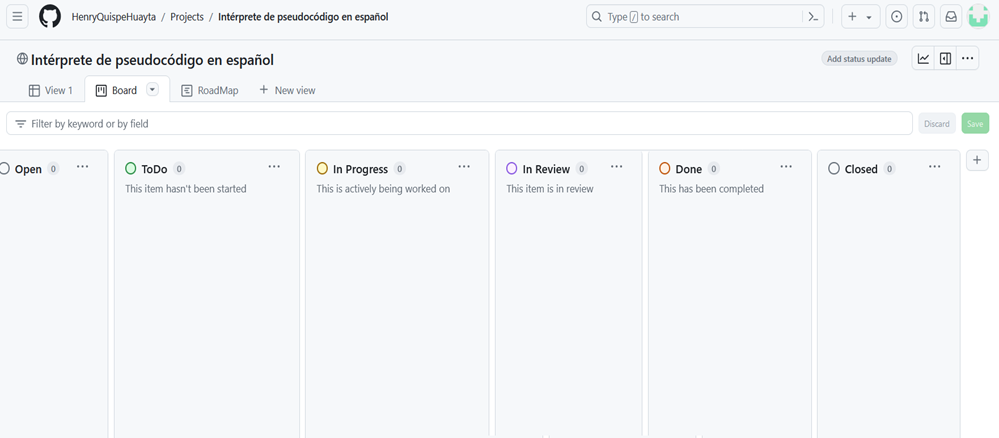
\includegraphics[width=1\textwidth]{images/tablero.png}
  \caption{Tablero de trabajo}
  \centering Fuente: Elaboración propia (GitHub)
  \label{fig:tablero}
\end{figure}
\newline
\newline
\newline

Se tiene un total de seis columnas, las cuales son:
\begin{itemize}
  \item \textbf{Open} \\
  Estas son las tareas que se han identificado inicialmente, que pueden incluir la creación de nuevas funcionalidades, corrección de errores, refactorizaciones, etc. Estas tareas están por definirse si van a ser atendidas o no. En esta etapa, se evalúa su importancia y se priorizan en función de las necesidades del proyecto.
  \item \textbf{ToDo} \\
  En esta columna del tablero se mueven las tareas que están listas para ser iniciadas. Aunque estas tareas aún no se están trabajando activamente, se encuentran en espera para su ejecución. Se aborda en función de su prioridad.
  \item \textbf{In Progress} \\
  Las tareas que se encuentran en esta columna ya están siendo trabajadas activamente. Aquí es donde se lleva a cabo la implementación de las funcionalidades o las correcciones de errores planificadas. Se monitorea el progreso de estas tareas para garantizar que avancen de manera eficiente.
  \item \textbf{In Review} \\
  Esta columna alberga las tareas que están en proceso de revisión. Una vez que una tarea ha sido completada, se somete a un proceso de revisión para garantizar la calidad del trabajo realizado. Si se encuentra algún error durante la revisión, la tarea se devuelve a la columna "In Progress" para su corrección.
  \item \textbf{Done} \\
  Una vez que una tarea ha pasado exitosamente por el proceso de revisión, se mueve a esta columna. Esto indica que la tarea ha sido completada satisfactoriamente. Las tareas permanecen en esta columna durante un tiempo antes de pasar a la columna final, en posible espera de algún cambio que requiera volver a una columna anterior.
  \item \textbf{Closed} \\
  En esta etapa final, las tareas que no requieren más trabajo o modificaciones se cierran. Esto puede incluir tareas que han sido completadas exitosamente y revisadas, así como aquellas que fueron abiertas pero finalmente decididas que no serán abordadas. Las tareas cerradas se archivan y ya no son parte del flujo de trabajo activo.
\end{itemize}

\subsection{Actividades}
Las principales actividades que se realizaron se registraron en el tablero Kanban, en la primera columna (Open).

\begin{itemize}
  \item \textbf{Implementation of Lexer (Implementación del Analizador Léxico).} \\
  Se implementó el analizador léxico del intérprete, que convirtió el código fuente en una secuencia de tokens según las reglas léxicas del lenguaje. Este componente escaneó el código y generó una lista estructurada de tokens, que fueron utilizados como entrada para las etapas posteriores del proceso de interpretación.
  \item \textbf{Implementation of Parser (Implementación del Analizador Sintáctico).} \\
  Durante esta fase, se desarrolló el analizador sintáctico que verificó la estructura gramatical del código fuente generado por el analizador léxico. El analizador sintáctico transformó la secuencia de tokens en un árbol de sintaxis abstracta (AST), asegurando que el código siguiera las reglas sintácticas del intérprete.
  \item \textbf{Interpreter Development and Code Execution (Desarrollo del Intérprete y Ejecución de Código).} \\
  Se completó la implementación del intérprete que utilizó el AST generado por el analizador sintáctico para ejecutar el programa. El intérprete interpretó cada nodo del AST y ejecutó las operaciones definidas por el código fuente, facilitando la ejecución del programa en tiempo real. \\
  \item \textbf{Error Handling (Manejo de Errores).} \\
  Durante esta etapa, se implementó un sistema completo de manejo de errores que detectó y gestionó problemas como errores de sintaxis, referencias a variables no definidas, y operaciones inválidas. Se proporcionaron mensajes de error detallados y personalizados para mejorar la experiencia del usuario y facilitar la depuración del código.
  \item \textbf{Context and Scope Management (Gestión de Contexto y Ámbito).} \\
  Se definió y se implementó cómo se almacenaron y accedieron variables y funciones dentro de diferentes contextos durante la ejecución del programa. La gestión adecuada de ámbitos aseguró que las variables locales y globales se manejan correctamente, contribuyendo a la correcta ejecución y funcionamiento del intérprete.
  \item \textbf{Definition of Built-in Constants and Values (Definición de Constantes y Valores Integrados).} \\
  Como fase final, se definieron y se implementaron las palabras clave, funciones integradas, constantes predefinidas y mensajes de error estándar del lenguaje. Estos elementos proporcionan la base fundamental para la funcionalidad básica del intérprete, permitiendo a los usuarios utilizar y gestionar de manera efectiva los recursos del lenguaje de programación implementado.
\end{itemize}

\begin{figure}[!h]
  \centering
  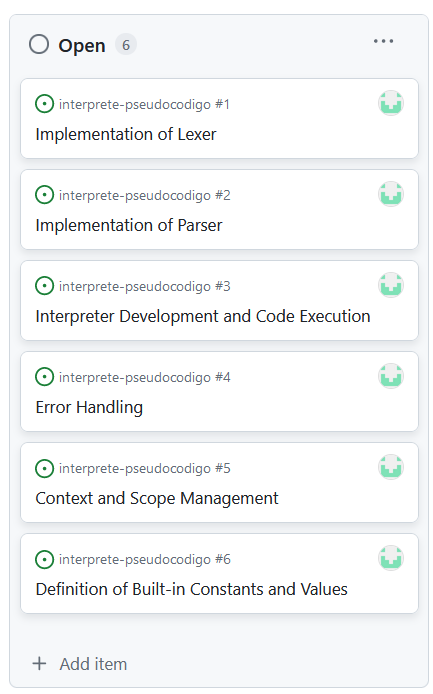
\includegraphics[width=0.6\textwidth]{images/actividades.png}
  \caption{Actividades realizadas}
  \centering Fuente: Elaboración propia (GitHub)
  \label{fig:actividades}
\end{figure}

\section{Análisis léxico}
\subsection{Lexemas y tokens}
Los Lexemas son el conjunto de palabras reservadas, signos, operadores y separadores, las palabras reservadas son palabras clave que no se pueden utilizar como identificadores, los signos y operadores sirven para realizar las operaciones y los separadores nos permiten indicar dónde comienza y termina cada uno de nuestros lexemas y la gramática en sí.
\begin{center}
  \begin{longtable}{|l|m{10em}|m{14em}|}
    \hline
    \textbf{Token} & \textbf{Descripción} & \textbf{Estructura o Formato Esperado} \\
    \hline
    \endfirsthead
    \hline
    \endhead
    \endfoot
    \hline
    TT\_INT & Tipo de dato entero & Números entero en base 10 \\
    \hline
    TT\_FLOAT & Tipo de dato real & Número decimal con punto flotante \\
    \hline
    TT\_STRING & Tipo de dato cadena & Cadena delimitada por comillas dobles \\
    \hline
    TT\_IDENTIFIER & Identificador & Nombres de variables y funciones \\
    \hline
    TT\_KEYWORD & Palabra clave & Palabra reservada del lenguaje \\
    \hline
    TT\_PLUS & Operador suma & Signo + \\
    \hline
    TT\_MINUS & Operador suma & Signo - \\
    \hline
    TT\_MUL & Operador multiplicación & Signo * \\
    \hline
    TT\_DIV & Operador división & Signo / \\
    \hline
    TT\_MOD & Operador módulo & Signo \% \\
    \hline
    TT\_POW & Operador potencia & Operador de potencia, ** \\
    \hline
    TT\_EQ & Operador igualdad & Operador de asignación o igualdad, = \\
    \hline
    TT\_LPAREN & Paréntesis izquierdo & Paréntesis de apertura, ( \\
    \hline
    TT\_RPAREN & Paréntesis derecho & Paréntesis de cierre, ) \\
    \hline
    TT\_LSQUARE & Corchete izquierdo & Corchete de apertura, [ \\
    \hline
    TT\_RSQUARE & Corchete derecho & Corchete de cierre, ] \\
    \hline
    TT\_EE & Operador igualdad estricta & Operador de comparación estricta de igualdad, == \\
    \hline
    TT\_MM & Operador decremento & Operador de decremento, -- \\
    \hline
    TT\_NE &Operador no igual &Operador de comparación de no igualdad, != \\
    \hline
    TT\_LT & Operador menor que & Operador de comparación menor que, < \\
    \hline
    TT\_GT & Operador mayor que & Operador de comparación mayor que, > \\
    \hline
    TT\_LTE & Operador menor o igual que & Operador de comparación menor o igual que, <= \\
    \hline
    TT\_GTE & Operador mayor o igual que & Operador de comparación mayor o igual que, >= \\
    \hline
    TT\_COMMA & Coma & Carácter de coma , \\
    \hline
    TT\_NEWLINE & Nueva línea & Carácter de salto de línea, \textbackslash n \\
    \hline
    TT\_EOF & Fin de archivo & N/A \\
    \hline
    \caption{Tokens. Tipos básicos}
  \end{longtable}
  \vspace*{-4.5em}
  \centering Fuente: Elaboración propia
\end{center}

Además de los tokens básicos, están las palabras reservadas específicas del intérprete:
\begin{table}[!h]
  \begin{center}
    \begin{tabularx}{0.9\textwidth}{|X|X|X|}
      \hline
      \textbf{Lexema} & \textbf{Descripción} & \textbf{Palabra Clave} \\
      \hline
      var & Variable & var \\
      \hline
      print & Mostrar en consola & imprimir \\
      \hline
      if & Condición si & si \\
      \hline
      then & Instrucción entonces & entonces \\
      \hline
      else & Instrucción sino & sino \\
      \hline
      elif & Instrucción osi & osi \\
      \hline
      end & Fin condición si & fin \\
      \hline
      while & Bucle mientras & mientras \\
      \hline
      then & Instrucción entonces & entonces \\
      \hline
      end & Fin bucle mientras & fin \\
      \hline
      in & Instrucción hasta & hasta \\
      \hline
      for & Bucle para & para \\
      \hline
      end & Fin bucle para & fin \\
      \hline
      function & Inicio función & funcion \\
      \hline
      end & Fin función & fin \\
      \hline
    \end{tabularx}
  \end{center}
  \caption{Lexemas y palabras reservadas}
  \centering Fuente: Elaboración propia
  \label{tab:lexemas}
\end{table}

\subsection{Autómatas individuales}
Los autómatas individuales son utilizados para representar gráficamente la secuencia de caracteres de las palabras reservadas, los signos y los operadores de nuestra gramática. Cada tipo de token puede ser representado mediante un autómata finito que define su estructura.

A continuación, en la Tabla \ref{tab:automatas}, se presentan los autómatas individuales para los tipos de tokens básicos del intérprete. Cada autómata describe la estructura y el formato esperado de los lexemas correspondientes, lo que permite identificar y clasificar los tokens durante el análisis léxico.
\begin{center}
  \begin{longtable}{|l|l|}
    \hline
    \multicolumn{1}{|l|}{\textbf{Tipo de Token}} & \multicolumn{1}{l|}{\textbf{Descripción Token}} \\
    \hline
    \endfirsthead
    \hline
    \endhead
    \hline
    \endfoot
    \endlastfoot
    TT\_INT, TT\_FLOAT & Tipo de dato entero y real \\
    \hline
    \multicolumn{2}{|l|}{} \\
    \multicolumn{2}{|c|}{
      \begin{minipage}{0.95\textwidth}
        \centering
        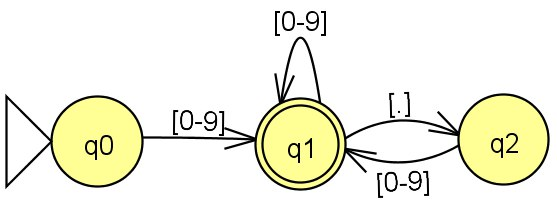
\includegraphics[width=0.6\textwidth]{images/number.png} \\[2ex]
        \begin{math}
          \begin{array}{rl}
            q0 & = [0-9] \, q1 \\
            q1 & = [0-9]^{*} + [.] \, q2 + \lambda \\
            q2 & = [0-9] \\
            ER & = [0-9]([0-9]+[.][0-9])^{*}
          \end{array}
        \end{math}
      \end{minipage}
    } \\
    \multicolumn{2}{|l|}{Estado inicial: q0} \\
    \multicolumn{2}{|l|}{
      \begin{minipage}{0.9\textwidth
      }
        \textbf{Transiciones:}
        \vspace*{-0.8em}
        \begin{itemize}
          \item Desde el estado q0 se requiere un dígito $([0-9])$ para poder pasar al estado q1.
          \item En el estado q1, puede haber un número indefinido de dígitos $([0-9])$ y finalizar sin pasar al estado q2.
          \item Puede haber un punto decimal $(.)$ que lleva al estado q2.
          \item En el estado q2, debe haber al menos un dígito $([0-9])$ después del punto decimal $(.)$ que lleva al estado q1.
        \end{itemize}
      \end{minipage}
    } \\
    \multicolumn{2}{|l|}{Estado final: q1 es el estado final válido.} \\
    \hline
    TT\_STRING & Tipo de dato cadena \\
    \hline
    \multicolumn{2}{|l|}{} \\
    \multicolumn{2}{|c|}{
      \begin{minipage}{0.95\textwidth}
        \centering
        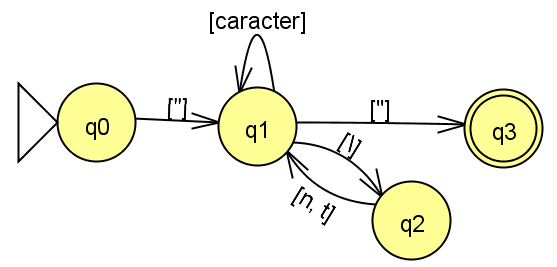
\includegraphics[width=0.6\textwidth]{images/string.png} \\[2ex]
        \begin{math}
          \begin{array}{rl}
            q0 & = ["] \, q1 \\
            q1 & = [caracter] q1 + [\backslash] \, q2 + ["] \, q3 \\
            q2 & = ([n] + [t]) \, q1 \\
            q3 & = \lambda \\
            ER & = ["]([caracter])^{*} ["] \, + \\
            & \quad ["][caracter]^{*} [\backslash] (([t]+[n])[caracter]^{*}[\backslash])^{*} ([t]+[n])[caracter]^{*} ["]
          \end{array}
        \end{math}
      \end{minipage}
    } \\
    \multicolumn{2}{|l|}{Estado inicial: q0} \\
    \multicolumn{2}{|l|}{
      \begin{minipage}{0.9\textwidth
      }
        \textbf{Transiciones:}
        \vspace*{-1.5em}
        \begin{itemize}
          \item Comienza con una comilla doble $(")$, pasa al estado q1.
          \item En el estado q1, puede haber cualquier carácter $([caracter])$, seguido por más caracteres o secuencias de escape como \textbackslash n o \textbackslash t.
          \item Se permite un número indefinido de repeticiones de caracteres y secuencias de escape.
          \item Termina con otra comilla doble $(")$, llegando al estado final q3.
        \end{itemize}
      \end{minipage}
    } \\
    \multicolumn{2}{|l|}{Estado final: q3 es el estado final válido.} \\
    \hline
    TT\_EQ, TT\_EE & Operador igualdad y comparación estricta \\
    \hline
    \multicolumn{2}{|l|}{} \\
    \multicolumn{2}{|c|}{
      \begin{minipage}{0.95\textwidth}
        \centering
        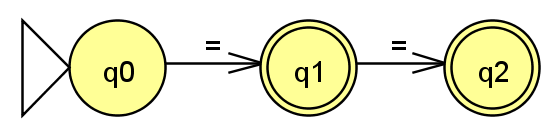
\includegraphics[width=0.6\textwidth]{images/equal.png} \\[2ex]
        \begin{math}
          \begin{array}{rl}
            q0 & = [=] \, q1 \\
            q1 & = ([=] + \lambda)\, q2 \\
            q2 & = \lambda \\
            ER & = [=]([=] + \lambda)
          \end{array}
        \end{math}
      \end{minipage}
    } \\
    \multicolumn{2}{|l|}{Estado inicial: q0} \\
    \multicolumn{2}{|l|}{
      \begin{minipage}{0.9\textwidth
      }
        \textbf{Transiciones:}
        \vspace*{-1.5em}
        \begin{itemize}
          \item Un solo símbolo de igual (=) lleva al estado final q1.
        \end{itemize}
      \end{minipage}
    } \\
    \multicolumn{2}{|l|}{Estado final: q2 es el estado final válido.} \\
    \hline
    TT\_NE & Operador no igual \\
    \hline
    \multicolumn{2}{|l|}{} \\
    \multicolumn{2}{|c|}{
      \begin{minipage}{0.95\textwidth}
        \centering
        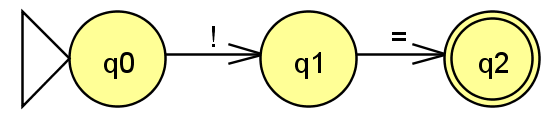
\includegraphics[width=0.6\textwidth]{images/notEqual.png} \\[2ex]
        \begin{math}
          \begin{array}{rl}
            q0 & = [!] \, q1 \\
            q1 & = [=] \, q2 \\
            q2 & = \lambda \\
            ER & = [!][=]
          \end{array}
        \end{math}
      \end{minipage}
    } \\
    \multicolumn{2}{|l|}{Estado inicial: q0} \\
    \multicolumn{2}{|l|}{
      \begin{minipage}{0.9\textwidth
      }
        \textbf{Transiciones:}
        \vspace*{-1.5em}
        \begin{itemize}
          \item Un signo de exclamación (!) seguido de un signo de igual (=) lleva al estado final q2.
        \end{itemize}
      \end{minipage}
    } \\
    \multicolumn{2}{|l|}{Estado final: q2 es el estado final válido.} \\
    \hline
    TT\_GT, TT\_GTE & Operador mayor que y mayor o igual que \\
    \hline
    \multicolumn{2}{|l|}{} \\
    \multicolumn{2}{|c|}{
      \begin{minipage}{0.95\textwidth}
        \centering
        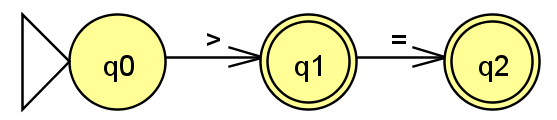
\includegraphics[width=0.6\textwidth]{images/greater.png} \\[2ex]
        \begin{math}
          \begin{array}{rl}
            q0 & = [>] \, q1 \\
            q1 & = ([=] + \lambda) \, q2 \\
            q2 & = \lambda \\
            ER & = [>]([=] + \lambda)
          \end{array}
        \end{math}
      \end{minipage}
    } \\
    \multicolumn{2}{|l|}{Estado inicial: q0} \\
    \multicolumn{2}{|l|}{
      \begin{minipage}{0.9\textwidth
      }
        \textbf{Transiciones:}
        \vspace*{-1.5em}
        \begin{itemize}
          \item Un solo signo de mayor que (>), seguido opcionalmente de un signo de igual (=), lleva al estado final q2.
        \end{itemize}
      \end{minipage}
    } \\
    \multicolumn{2}{|l|}{Estado final: q2 es el estado final válido.} \\
    \hline
    TT\_LT, TT\_LTE & Operador menor que y menor o igual que \\
    \hline
    \multicolumn{2}{|c|}{
      \begin{minipage}{0.95\textwidth}
        \centering
        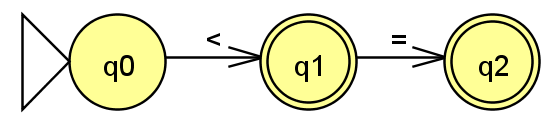
\includegraphics[width=0.6\textwidth]{images/less.png} \\[2ex]
        \begin{math}
          \begin{array}{rl}
            q0 & = [<] \, q1 \\
            q1 & = ([=] + \lambda) \, q2 \\
            q2 & = \lambda \\
            ER & = [<]([=] + \lambda)
          \end{array}
        \end{math}
      \end{minipage}
    } \\
    \multicolumn{2}{|l|}{Estado inicial: q0} \\
    \multicolumn{2}{|l|}{
      \begin{minipage}{0.9\textwidth
      }
        \textbf{Transiciones:}
        \vspace*{-1.5em}
        \begin{itemize}
          \item Un solo signo de menor que (<), seguido opcionalmente de un signo de igual (=), lleva al estado final q2.
        \end{itemize}
      \end{minipage}
    } \\
    \multicolumn{2}{|l|}{Estado final: q2 es el estado final válido.} \\
    \hline
    \caption{Autómatas individuales}
    \label{tab:automatas}
  \end{longtable}
  \vspace*{-4.5em}
  \centering Fuente: Elaboración propia
\end{center}

\section{Análisis sintáctico}
\subsection{Gramática BNF}
Cada regla de la gramática BNF se compone de símbolos no terminales y terminales, donde los símbolos no terminales representan categorías sintácticas que pueden expandirse en otras reglas, mientras que los símbolos terminales son los elementos léxicos fundamentales del lenguaje.

Para las distintas Palabras claves (Keywords) que tiene el intérprete sus gramáticas serían las siguientes:

\begin{itemize}
  \item \textbf{IF-THEN-END} \\
  \begin{math}
    \begin{array}{rl}
      <instruccion> & ::= Keywords.IF <expresion> Keywords.THEN \\ 
        & \quad <lista\_instrucciones> Keywords.END
    \end{array}
  \end{math} \\\\
  Define una estructura condicional que comienza con si, seguida de una condición $(<expresion>)$, un bloque de instrucciones $(<lista\_instrucciones>)$ y termina con fin. Se usa para ejecutar un bloque de código si se cumple una condición.
  \item \textbf{ELSEIF y ELSE} \\
  \begin{math}
    \begin{array}{rl}
      <caso> & ::= Keywords.ELSEIF <expresion> Keywords.THEN \\
        & \quad <lista\_instrucciones> <inst\_parar> \\
      <caso> & ::= Keywords.ELSE : <lista\_instrucciones> <inst\_parar>
    \end{array}
  \end{math} \\\\
  ELSEIF se utiliza para añadir una condición alternativa a una estructura IF, mientras que ELSE se usa para ejecutar un bloque de código si ninguna de las condiciones anteriores se cumple.
  \item \textbf{FOR-TO-STEP} \\
  \begin{math}
    \begin{array}{rl}
      <inst\_para> & ::= Keywords.FOR <inst\_asignacion> Keywords.TO \\
        & \quad <expresion> [Keywords.STEP <expresion>] \\ 
        & \quad Keywords.THEN <lista\_instrucciones> \\
        & \quad Keywords.END
    \end{array}
  \end{math} \\\\
  Define un bucle for que inicializa una variable $(<inst\_asignacion>)$, especifica una condición de terminación $(TO <expresion>)$, y opcionalmente un paso $(STEP <expresion>)$, ejecutando un bloque de código repetidamente hasta que se cumpla la condición de terminación.
  \item \textbf{WHILE-END} \\
  \begin{math}
    \begin{array}{rl}
      <inst\_mientras> & ::= Keywords.WHILE <expresion> \\
        & \quad Keywords.THEN <lista\_instrucciones> \\
        & \quad Keywords.END
    \end{array}
  \end{math} \\\\
  Define un bucle while que ejecuta un bloque de código mientras se cumpla una condición $(<expresion>)$, terminando cuando la condición ya no se cumple.
  \item \textbf{FUNCTION-END} \\
  \begin{math}
    \begin{array}{rl}
      <inst\_funcion> & ::= Keywords.FUNCTION <identificador> \\
        & \quad Keywords.THEN <lista\_instrucciones> \\
        & \quad Keywords.END
    \end{array}
  \end{math} \\\\
  Define la estructura que comienza con función, seguida de un $(<identificador>)$, un bloque de instrucciones $(<lista\_instrucciones>)$ y termina con fin. Se utiliza para definir una función personalizada que puede ser llamada en otras partes del código.
  \item \textbf{VAR} \\
  \begin{math}
    \begin{array}{rl}
      <inst\_variable> & ::= Keywords.VAR <identificador> \\
      & \quad Keywords.EQ <expresion>
    \end{array}
  \end{math} \\\\
  Define una instrucción de asignación que comienza con var, seguida de un $(<identificador>)$, un signo de igualdad $(Keywords.EQ)$ y una $(<expresion>)$ que se asigna a la variable.
  \item \textbf{RETURN} \\
  \begin{math}
    \begin{array}{rl}
      <inst\_retorno> & ::= Keywords.RETURN <expresion>
    \end{array}
  \end{math} \\\\
  Define una instrucción de retorno que comienza con return, seguida de una $(<expresion>)$ que se devuelve como resultado de la función o para salir de un bucle.
  \item \textbf{CONTINUE y BREAK} \\
  \begin{math}
    \begin{array}{rl}
      <inst\_continuar> & ::= Keywords.CONTINUE \\
      <inst\_parar> & ::= Keywords.BREAK
    \end{array}
  \end{math} \\\\
  CONTINUE se utiliza para saltar a la siguiente iteración de un bucle, mientras que BREAK se usa para salir de un bucle antes de que se complete.
  \item \textbf{PRINT} \\
  \begin{math}
    \begin{array}{rl}
      <inst\_imprimir> & ::= Keywords.PRINT (<expresion>)
    \end{array}
  \end{math} \\\\
  Define una instrucción de impresión que comienza con imprimir, seguida de una $(<expresion>)$ que se muestra en la consola.
\end{itemize}

\subsection{Primeros}
Los primeros de una gramática son los símbolos no terminales que pueden aparecer en la parte izquierda de una producción. Los primeros determinan qué símbolos pueden comenzar una cadena derivada de un símbolo no terminal. Para la gramática del intérprete, los primeros de cada no terminal son los siguientes:
\begin{table}[!h]
  \begin{center}
    \begin{tabularx}{1\textwidth}{|X|X|}
      \hline
      \textbf{No Terminal} & \textbf{Primeros} \\
      \hline
      <instruccion> & Keywords.IF, Keywords.WHILE, Keywords.FOR, Keywords.FUNCTION, Keywords.VAR, Keywords.RETURN, Keywords.CONTINUE, Keywords.BREAK, Keywords.PRINT, Identificador \\
      \hline
      <caso> & Keywords.ELSEIF, Keywords.ELSE \\
      \hline
      <inst\_para> & Keywords.FOR \\
      \hline
      <inst\_mientras> & Keywords.WHILE \\
      \hline
      <inst\_funcion> & Keywords.FUNCTION \\
      \hline
      <inst\_variable> & Keywords.VAR \\
      \hline
      <inst\_retorno> & Keywords.RETURN \\
      \hline
      <inst\_continuar> & Keywords.CONTINUE \\
      \hline
      <inst\_parar> & Keywords.BREAK \\
      \hline
      <inst\_imprimir> & Keywords.PRINT \\
      \hline
    \end{tabularx}
  \end{center}
  \caption{Primeros de la gramática}
  \centering Fuente: Elaboración propia
  \label{tab:primeros}
\end{table}

\subsection{Siguientes}
Los siguientes de una gramática son los símbolos no terminales que pueden aparecer inmediatamente después de un símbolo no terminal en una cadena derivada. Los siguientes determinan qué símbolos pueden seguir a un no terminal en una derivación. Para la gramática del intérprete, los siguientes de cada no terminal son los siguientes:
\begin{table}[!h]
  \begin{center}
    \begin{tabularx}{1\textwidth}{|X|X|}
      \hline
      \textbf{No Terminal} & \textbf{Siguientes} \\
      \hline
      <instruccion> & Keywords.END, Identificador \\
      \hline
      <caso> & Keywords.END, Keywords.ELSEIF, Keywords.ELSE \\
      \hline
      <inst\_para> & Keywords.END, Identificador \\
      \hline
      <inst\_mientras> & Keywords.END, Identificador \\
      \hline
      <inst\_funcion> & Keywords.END, Identificador \\
      \hline
      <inst\_variable> & Keywords.END, Identificador \\
      \hline
      <inst\_retorno> & Keywords.END, Identificador \\
      \hline
      <inst\_continuar> & Keywords.END, Identificador \\
      \hline
      <inst\_parar> & Keywords.END, Identificador \\
      \hline
      <inst\_imprimir> & Keywords.END, Identificador \\
      \hline
    \end{tabularx}
  \end{center}
  \caption{Siguientes de la gramática}
  \centering Fuente: Elaboración propia
  \label{tab:siguientes}
\end{table}

\section{Análisis semántico}
El análisis semántico es una etapa crucial en el proceso de compilación e interpretación que verifica la corrección semántica del código fuente después de haber pasado por el análisis léxico y sintáctico. La implementación del análisis semántico se realizó siguiendo estos puntos:

\subsection{Definición de Contextos y Alcance}
\begin{itemize}
  \item Se definieron contextos que guardan información sobre el alcance actual, incluyendo variables, funciones y otros identificadores visibles.
  \item Los contextos permitieron la gestión de scopes, soportando características como variables locales y globales, y la resolución de nombres.
\end{itemize}

\subsection{Verificación de Tipos}
\begin{itemize}
  \item Se implementaron reglas para verificar que las operaciones realizadas sobre los datos fueran semánticamente válidas. Por ejemplo, no se permitía sumar una cadena con un número.
  \item Se verificó que las funciones se llamaran con los tipos y cantidad correctos de argumentos.
\end{itemize}

\section{Evaluación y Ejecución}
\subsection{Evaluación}
El intérprete lee y analiza el contenido del archivo .inf. Durante este proceso, identifica y carga todas las variables, funciones y configuraciones definidas en el archivo. Este paso asegura que todos los elementos necesarios para la ejecución del programa estén disponibles.

Verifica las reglas semánticas definidas internamente y aplicadas en el archivo .inf. Por ejemplo, puede asegurarse de que las variables estén correctamente declaradas y que las funciones estén bien definidas según las reglas gramaticales y semánticas del intérprete.

\subsection{Ejecución}
Una vez completada la evaluación semántica y cargadas todas las configuraciones necesarias desde el archivo .inf, el intérprete procede a ejecutar el programa principal.

El intérprete ejecuta las instrucciones secuenciales definidas en el programa principal. Durante este proceso, el intérprete puede modificar el estado de las variables, realizar cálculos, llamar a funciones definidas previamente, y mostrar información en pantalla.

Una vez que todas las instrucciones del programa principal han sido ejecutadas, el intérprete completa su ejecución. En este punto, puede devolver un resultado final al usuario, mostrar información en pantalla, o realizar cualquier acción definida por el programa.

Durante la ejecución, el intérprete también maneja posibles errores que puedan surgir, como errores de sintaxis, errores de tiempo de ejecución (como divisiones por cero o acceso a memoria no válida), o excepciones específicas del lenguaje. La gestión adecuada de errores asegura que el programa pueda responder de manera apropiada ante situaciones inesperadas.

\chapter{PRUEBAS Y RESULTADOS}
En esta fase del proyecto, se llevaron a cabo diversas pruebas para comprobar el correcto funcionamiento y verificar la calidad del intérprete, basándonos en los ocho puntos definidos por la norma ISO 25010. Para asegurar que el intérprete cumple con los estándares de calidad, se realizaron encuestas a los usuarios y pruebas directas al intérprete.

\section{Funcionalidad}
Esta prueba evalúa si el intérprete cumple con sus funciones básicas y requerimientos especificados.

Para esta prueba usamos una parte de la encuesta realizada a los usuarios que probaron el intérprete. Con esta verificamos si se encontraron errores durante la ejecución.
\begin{table}[!h]
  \begin{center}
    \begin{tabularx}{0.9\textwidth}{|X|X|}
      \hline
      \textbf{Pregunta} & \textbf{Descripción} \\
      \hline
      ¿Encontró algún error o problema técnico durante el uso del intérprete? & Esta pregunta identifica fallos funcionales. \\
      \hline
      Si respondió ``Sí'' en la pregunta anterior, por favor detalle el problema: & Los detalles aquí proporcionados serán utilizados para identificar problemas específicos y áreas que necesitan mejoras. \\
      \hline
    \end{tabularx}
  \end{center}
  \caption{Partes de la encuesta de funcionalidad}
  \centering Fuente: Elaboración propia
  \label{tab:funcionalidad}
\end{table}

Para esta prueba usamos una parte de la encuesta realizada a los usuarios que probaron el intérprete. Con esta verificamos si se encontraron errores durante la ejecución.

La Eficiencia en la Eliminación de Defectos (EED) es una medida utilizada en la gestión de la calidad para evaluar cuántos defectos se eliminan en relación con el esfuerzo total invertido en la detección y corrección de esos defectos. Se calcula utilizando la siguiente fórmula:
\begin{equation*}
  \begin{split}
    EED = \frac{(D - D_r)}{D} \times 100\%
  \end{split}
\end{equation*}

Donde:
\begin{equation*}
  \begin{split}
    D & \quad \textnormal{Es el número total de defectos antes de la corrección.}\\
    D_r & \quad \textnormal{Es el número de defectos restantes después de la corrección.}
  \end{split}
\end{equation*}

Antes de pasar a la etapa de pruebas con el software se encontraron los siguientes errores.

\begin{itemize}
  \item Error en la comparación de variables.
  \item Error en asignación de variables con ñ.
  \item Ejecución del bucle infinito en algunas ejecuciones de para (for).
  \item Error al cerrar una función.
  \item No se puede re-asignar una variable.
  \item No reconoce el salto de línea.
  \item Error al tener un si (if) dentro de un para (for).
  \item Error durante la instalación del intérprete.
  \item No se agrega al path de las variables de entorno.
\end{itemize}

Previamente se presentaron estos 9 errores.

Durante la recolección de datos, los usuarios reportaron este problema.
\begin{itemize}
  \item El poder instalar, porque se bloqueaba al descargar.
  \item No corre poniendo el comando dado en la terminal o tal vez no está muy  bien explicado.
\end{itemize}

De estos reportes, uno hace referencia a los errores previos y de funcionalidad.

Por lo tanto, tenemos que:
\begin{equation*}
  \begin{split}
    EED & = \frac{(9 - 1)}{9} \times 100\% \\
    EED & = 88.89 \%
  \end{split}
\end{equation*}

Por lo se deduce que se cuenta con una funcionalidad aceptable y también se debe trabajar en un error nuevo que se presentó, relacionado con la comprensión de la documentación.

\section{Fiabilidad}
Esta prueba evalúa la estabilidad y consistencia del intérprete bajo condiciones de uso normales.

Para esta prueba usamos una parte de la encuesta realizada a los usuarios que probaron el intérprete. Con esta calificamos la experiencia con el intérprete.
\begin{table}[!h]
  \begin{center}
    \begin{tabularx}{0.9\textwidth}{|X|X|}
      \hline
      \textbf{Pregunta} & \textbf{Descripción} \\
      \hline
      ¿Cuál fue su experiencia con el intérprete? & Permite evaluar la percepción general sobre la fiabilidad del intérprete. \\
      \hline
    \end{tabularx}
  \end{center}
  \caption{Partes de la encuesta, fiabilidad}
  \centering Fuente: Elaboración propia
  \label{tab:fiabilidad}
\end{table}

A continuación se muestra la escala de valores utilizada para evaluar la fiabilidad. Esta escala considera diferentes niveles, cada uno asociado con un valor específico y la cantidad correspondiente de casos evaluados.
\begin{table}[!h]
  \begin{center}
    \begin{tabularx}{0.9\textwidth}{|X|X|X|}
      \hline
      \textbf{Escala} & \textbf{Valor} & \textbf{Cantidad} \\
      \hline
      Muy buena & 5 & 15 \\
      \hline
      Buena & 4 & 25 \\
      \hline
      Regular & 3 & 12 \\
      \hline
      Mala & 2 & 1 \\
      \hline
      Muy mala & 1 & 0 \\
      \hline
    \end{tabularx}
  \end{center}
  \caption{Escala de valores para la fiabilidad}
  \centering Fuente: Elaboración propia
  \label{tab:fiabilidad-escala}
\end{table}

Realizando una media de los datos obtenidos tenemos:
\begin{equation*}
  \begin{split}
    \textnormal{Fiabilidad} & = \frac{\sum (\textnormal{valor} \times \textnormal{cantidad})}{5 \times \sum \textnormal{cantidad}} \times 100\% \\
    \textnormal{Fiabilidad} & = \frac{(5 \times 15 + 4 \times 25 + 3 \times 12 \times 2)}{5 \times 53} \times 100\% \\
    \textnormal{Fiabilidad} & = 80.38\%
  \end{split}
\end{equation*}

Por lo tanto, se puede concluir que la fiabilidad del intérprete es buena. Sin embargo, se debe trabajar en mejorar la percepción de los usuarios.

\section{Usabilidad}
Esta prueba evalúa qué tan fácil y agradable es para los usuarios interactuar con el intérprete.

Para esta prueba usamos una parte de la encuesta realizada a los usuarios que probaron el intérprete. Con esta calificamos el nivel de usabilidad que tiene el intérprete.
\begin{table}[!h]
  \begin{center}
    \begin{tabularx}{0.9\textwidth}{|X|X|}
      \hline
      \textbf{Pregunta} & \textbf{Descripción} \\
      \hline
      ¿Cómo calificaría la facilidad de uso del intérprete? & Se centra en la experiencia directa con la interfaz del intérprete. \\
      \hline
    \end{tabularx}
  \end{center}
  \caption{Partes de la encuesta, usabilidad}
  \centering Fuente: Elaboración propia
  \label{tab:usabilidad}
\end{table}

A continuación se muestra la escala de valores utilizada para evaluar la usabilidad. Esta escala considera diferentes niveles, cada uno asociado con un valor específico y la cantidad correspondiente de casos evaluados.

\begin{table}[!h]
  \begin{center}
    \begin{tabularx}{0.9\textwidth}{|X|X|X|}
      \hline
      \textbf{Escala} & \textbf{Valor} & \textbf{Cantidad} \\
      \hline
      Muy fácil & 5 & 14 \\
      \hline
      Fácil & 4 & 22 \\
      \hline
      Regular & 3 & 17 \\
      \hline
      Difícil & 2 & 0 \\
      \hline
      Muy difícil & 1 & 0 \\
      \hline
    \end{tabularx}
  \end{center}
  \caption{Escala de valores para la usabilidad}
  \centering Fuente: Elaboración propia
  \label{tab:usabilidad-escala}
\end{table}

Realizando una media de los datos obtenidos tenemos:
\begin{equation*}
  \begin{split}
    \textnormal{Usabilidad} & = \frac{\sum (\textnormal{valor} \times \textnormal{cantidad})}{5 \times \sum \textnormal{cantidad}} \times 100\% \\
    \textnormal{Usabilidad} & = \frac{(5 \times 14 + 4 \times 22 + 3 \times 17)}{5 \times 53} \times 100\% \\
    \textnormal{Usabilidad} & = 78.87\%
  \end{split}
\end{equation*}

Por lo tanto, se puede concluir que la usabilidad del intérprete es buena. Sin embargo, se debe trabajar en mejorar la percepción de los usuarios.

\section{Eficiencia}
Esta prueba analiza el rendimiento del intérprete, incluyendo velocidad y consumo de recursos.

Para esta prueba usamos una parte de la encuesta realizada a los usuarios que probaron el intérprete. Con esta calificamos el nivel de eficiencia que presenta el intérprete.
\begin{table}[!h]
  \begin{center}
    \begin{tabularx}{0.9\textwidth}{|X|X|}
      \hline
      \textbf{Pregunta} & \textbf{Descripción} \\
      \hline
      ¿Qué tan rápido y eficiente considera que es el intérprete en su ejecución? & Esta pregunta proporciona una evaluación subjetiva de la eficiencia del intérprete. \\
      \hline
    \end{tabularx}
  \end{center}
  \caption{Partes de la encuesta, eficiencia}
  \centering Fuente: Elaboración propia
  \label{tab:eficiencia}
\end{table}
\newpage
A continuación se muestra la escala de valores utilizada para evaluar la eficiencia. Esta escala considera diferentes niveles, cada uno asociado con un valor específico y la cantidad correspondiente de casos evaluados.

\begin{table}[!h]
  \begin{center}
    \begin{tabularx}{0.9\textwidth}{|X|X|X|}
      \hline
      \textbf{Escala} & \textbf{Valor} & \textbf{Cantidad} \\
      \hline
      Muy rápido & 5 & 27 \\
      \hline
      Rápido & 4 & 24 \\
      \hline
      Regular & 3 & 2 \\
      \hline
      Lento & 2 & 0 \\
      \hline
      Muy lento & 1 & 0 \\
      \hline
    \end{tabularx}
  \end{center}
  \caption{Escala de valores para la eficiencia}
  \centering Fuente: Elaboración propia
  \label{tab:eficiencia-escala}
\end{table}

Realizando una media de los datos obtenidos tenemos:
\begin{equation*}
  \begin{split}
    \textnormal{Eficiencia} & = \frac{\sum (\textnormal{valor} \times \textnormal{cantidad})}{5 \times \sum \textnormal{cantidad}} \times 100\% \\
    \textnormal{Eficiencia} & = \frac{(5 \times 27 + 4 \times 24 + 3 \times 2)}{5 \times 53} \times 100\% \\
    \textnormal{Eficiencia} & = 89.43\%
  \end{split}
\end{equation*}

Por lo tanto, se puede concluir que la eficiencia del intérprete es muy buena. Sin embargo, se debe trabajar en mejorar la percepción de los usuarios.

\section{Mantenibilidad}
Para asegurar la mantenibilidad de nuestro proyecto según la norma ISO/IEC 25010, hemos implementado una documentación exhaustiva y una estructura de código modular y limpia. La documentación incluye guías de usuario, manuales técnicos y procedimientos de instalación que facilitan la comprensión y contribución al proyecto. Además, el código está diseñado con nombres descriptivos y comentarios claros, siguiendo las mejores prácticas de programación. Hemos establecido una cobertura de pruebas robusta con pruebas unitarias, de integración y de sistema, y utilizamos un sistema de control de versiones con Git, asegurando un flujo de trabajo eficiente con commits documentados y ramas claramente definidas.

\section{Portabilidad}
El intérprete puede ser instalado y utilizado de manera efectiva en diferentes sistemas operativos como Linux y Windows. Esta característica se logra mediante el uso de tecnologías y prácticas que aseguran su compatibilidad y rendimiento óptimo en ambas plataformas sin necesidad de modificaciones adicionales por parte del usuario.

\section{Seguridad}
Para garantizar la integridad del código, se emplearon las herramientas proporcionadas por GitHub:
\begin{itemize}
  \item \textbf{Gestión de Accesos y Colaboradores} \\
  Se configuraron cuidadosamente los permisos de acceso al repositorio.
  \item \textbf{Política de Revisión de Código} \\
  Se ha definido una política clara de revisión de código que asegura que todas las contribuciones enviadas mediante pull requests serán cuidadosamente revisadas antes de su integración en la rama principal del proyecto.
  \item \textbf{Gestión de Issues y Pull Requests} \\
  Se ha establecido un sistema de seguimiento de problemas y solicitudes de cambios que permite a los colaboradores reportar errores y proponer mejoras de manera segura y eficiente.
\end{itemize}

\begin{figure}[!h]
  \centering
  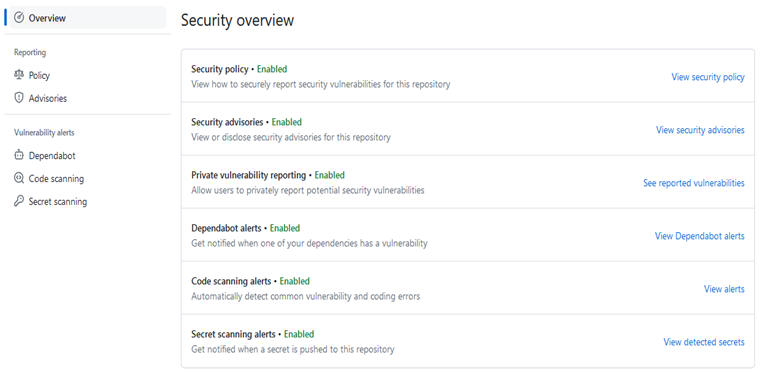
\includegraphics[width=0.8\textwidth]{images/seguridad.png}
  \caption{Seguridad}
  \centering Fuente: Elaboración propia
  \label{fig:seguridad}
\end{figure}

\section{Compatibilidad}
Se garantizó la compatibilidad del intérprete desarrollado mediante la implementación de la capacidad para ejecutar archivos exclusivos con extensión “.inf”. Estos archivos a su vez tienen una estructura clara, que se detalla en la documentación, si se sigue la estructura planteada y se le asigna la extensión adecuada, entonces se garantiza que el archivo es portable en cualquier sistema operativo que se encuentre instalado.

\section{Prueba de hipótesis}
\begin{itemize}
  \item \textbf{Variable Dependiente (VD):} La percepción media de los usuarios sobre la fiabilidad, usabilidad y eficiencia del intérprete.
  \item \textbf{Variable Independiente (VI):} El nivel aceptable $(3)$.
  \item \textbf{H0 (Hipótesis nula):} La percepción media de los usuarios sobre la fiabilidad, usabilidad y eficiencia del intérprete es igual o menor a un nivel aceptable $(3)$.
  \item \textbf{H1 (Hipótesis alternativa):} La percepción media de los usuarios sobre la fiabilidad, usabilidad y eficiencia del intérprete es mayor que un nivel aceptable $(>3)$.
\end{itemize}

\subsection{Prueba t de student}
La prueba t de una sola muestra compara la media de un solo grupo con un valor de referencia conocido.

\begin{center}
  \begin{longtable}{|l|l|l|l|}
    \hline
    & \textbf{Fiabilidad} & \textbf{Usabilidad} & \textbf{Eficiencia} \\
    \hline
    \endfirsthead
    \hline
    \endhead
    \endfoot
    \hline
    1 & 3 & 3 & 5 \\
    \hline
    2 & 3 & 3 & 3 \\
    \hline
    3 & 3 & 5 & 5 \\
    \hline
    4 & 4 & 3 & 5 \\
    \hline
    5 & 3 & 3 & 5 \\
    \hline
    6 & 3 & 3 & 5 \\
    \hline
    7 & 3 & 2 & 3 \\
    \hline
    8 & 3 & 3 & 4 \\
    \hline
    9 & 3 & 4 & 5 \\
    \hline
    10 & 3 & 4 & 5 \\
    \hline
    11 & 3 & 4 & 5 \\
    \hline
    12 & 3 & 3 & 5 \\
    \hline
    13 & 3 & 3 & 5 \\
    \hline
    14 & 4 & 4 & 4 \\
    \hline
    15 & 4 & 4 & 5 \\
    \hline
    16 & 4 & 4 & 4 \\
    \hline
    17 & 3 & 4 & 3 \\
    \hline
    18 & 4 & 3 & 5 \\
    \hline
    19 & 3 & 4 & 5 \\
    \hline
    20 & 3 & 3 & 4 \\
    \hline
    21 & 3 & 3 & 5 \\
    \hline
    22 & 3 & 3 & 4 \\
    \hline
    23 & 4 & 4 & 4 \\
    \hline
    24 & 5 & 5 & 5 \\
    \hline
    25 & 5 & 5 & 4 \\
    \hline
    26 & 5 & 5 & 5 \\
    \hline
    27 & 4 & 4 & 4 \\
    \hline
    28 & 4 & 4 & 4 \\
    \hline
    29 & 5 & 5 & 5 \\
    \hline
    30 & 5 & 5 & 5 \\
    \hline
    31 & 5 & 5 & 5 \\
    \hline
    32 & 5 & 5 & 5 \\
    \hline
    33 & 5 & 5 & 5 \\
    \hline
    34 & 5 & 5 & 5 \\
    \hline
    35 & 5 & 5 & 5 \\
    \hline
    36 & 4 & 4 & 4 \\
    \hline
    37 & 4 & 4 & 4 \\
    \hline
    38 & 5 & 5 & 5 \\
    \hline
    39 & 5 & 5 & 5 \\
    \hline
    40 & 4 & 4 & 4 \\
    \hline
    41 & 4 & 4 & 4 \\
    \hline
    42 & 4 & 4 & 4 \\
    \hline
    43 & 5 & 5 & 5 \\
    \hline
    44 & 4 & 4 & 4 \\
    \hline
    45 & 4 & 4 & 4 \\
    \hline
    46 & 4 & 4 & 4 \\
    \hline
    47 & 4 & 4 & 4 \\
    \hline
    48 & 4 & 4 & 4 \\
    \hline
    49 & 4 & 4 & 4 \\
    \hline
    50 & 4 & 4 & 4 \\
    \hline
    51 & 4 & 4 & 4 \\
    \hline
    52 & 4 & 4 & 4 \\
    \hline
    53 & 5 & 5 & 5 \\
    \hline
    \caption{Resultado en la percepción de los usuarios}
  \end{longtable}
  \vspace*{-2.5em}
  \centering Fuente: Elaboración propia
\end{center}

Calcular la media global.
\begin{equation*}
  \begin{split}
    \overline{X} & = \frac{\sum_{i=1}^{n} x_i}{n} \\
    \overline{X} & = \frac{658}{159} \\
    \overline{X} & = 4.138
  \end{split}
\end{equation*}

Calcular las medias de cada grupo.
\begin{equation*}
  \begin{split}
    \overline{X}_j & = \frac{\sum_{i=1}^{n} x_{ij}}{n}
  \end{split}
\end{equation*}

Fiabilidad:
\begin{equation*}
  \begin{split}
    \overline{X}_{fiabilidad} & = \frac{209}{53} \\
    \overline{X}_{fiabilidad} & = 3.943
  \end{split}
\end{equation*}

Usabilidad:
\begin{equation*}
  \begin{split}
    \overline{X}_{usabilidad} & = \frac{213}{40} \\
    \overline{X}_{usabilidad} & = 4.019
  \end{split}
\end{equation*}

Eficiencia:
\begin{equation*}
  \begin{split}
    \overline{X}_{eficiencia} & = \frac{236}{66} \\
    \overline{X}_{eficiencia} & = 4.453
  \end{split}
\end{equation*}

Grados de libertad $(df)$.
\begin{equation*}
  \begin{split}
    df & = n - 1 \\
    df & = 53 - 1 \\
    df & = 52
  \end{split}
\end{equation*}

Desviación estándar muestral.

Fiabilidad:
\begin{equation*}
  \begin{split}
    S_{fiabilidad} & = \sqrt{\frac{\sum_{i=1}^{n} (x_{i} - \overline{X}_{fiabilidad})^2}{n - 1}} \\
    S_{fiabilidad} & = \sqrt{\frac{30.830}{52}} \\
    S_{fiabilidad} & = 0.770
  \end{split}
\end{equation*}

Usabilidad:
\begin{equation*}
  \begin{split}
    S_{usabilidad} & = \sqrt{\frac{\sum_{i=1}^{n} (x_{i} - \overline{X}_{usabilidad})^2}{n - 1}} \\
    S_{usabilidad} & = \sqrt{\frac{30.981}{52}} \\
    S_{usabilidad} & = 0.772
  \end{split}
\end{equation*}

Eficiencia:
\begin{equation*}
  \begin{split}
    S_{eficiencia} & = \sqrt{\frac{\sum_{i=1}^{n} (x_{i} - \overline{X}_{eficiencia})^2}{n - 1}} \\
    S_{eficiencia} & = \sqrt{\frac{19.132}{52}} \\
    S_{eficiencia} & = 0.607
  \end{split}
\end{equation*}

Estadístico t.
\begin{equation*}
  \begin{split}
    t & = \frac{\overline{X} - \mu_0}{\frac{S}{\sqrt{n}}} \\
  \end{split}
\end{equation*}

Fiabilidad:
\begin{equation*}
  \begin{split}
    t_{fiabilidad} & = \frac{3.943 - 3}{\frac{0.770}{\sqrt{53}}} \\
    t_{fiabilidad} & = 8.920
  \end{split}
\end{equation*}

Usabilidad:
\begin{equation*}
  \begin{split}
    t_{usabilidad} & = \frac{4.019 - 3}{\frac{0.772}{\sqrt{40}}} \\
    t_{usabilidad} & = 9.610
  \end{split}
\end{equation*}

Eficiencia:
\begin{equation*}
  \begin{split}
    t_{eficiencia} & = \frac{4.453 - 3}{\frac{0.607}{\sqrt{66}}} \\
    t_{eficiencia} & = 17.437
  \end{split}
\end{equation*}

Valor crítico p.

Fiabilidad:
\begin{equation*}
  \begin{split}
    p_{fiabilidad} & = (t=8.920, df=52) \\
    p_{fiabilidad} & = 2.311 \times 10^{-12}
  \end{split}
\end{equation*}

Usabilidad:
\begin{equation*}
  \begin{split}
    p_{usabilidad} & = (t=9.610, df=39) \\
    p_{usabilidad} & = 2.020 \times 10^{-13}
  \end{split}
\end{equation*}

Eficiencia:
\begin{equation*}
  \begin{split}
    p_{eficiencia} & = (t=17.437, df=65) \\
    p_{eficiencia} & = 1.123 \times 10^{-23}
  \end{split}
\end{equation*}

El valor $p$ es extremadamente bajo en todos los casos (menor que cualquier nivel común de significancia, como $0.05, 0.01 o 0.001$), lo que sugiere que se rechaza la hipótesis nula en cada caso y aceptamos la hipótesis alternativa. 

Por lo tanto, podemos concluir que la percepción media de los usuarios sobre la fiabilidad, usabilidad y eficiencia del intérprete es mayor que un nivel aceptable $(>3)$.

\chapter{CONCLUSIONES Y RECOMENDACIONES}

\section{Conclusiones}
De los resultados obtenidos llegamos a evidenciar el cumplimiento de todos los objetivos trazados en el presente trabajo de investigación, los cuales se resumen a continuación:
\begin{itemize}
  \item Se desarrolló un prototipo de intérprete de pseudocódigo en español para programación estructurada. Este prototipo permite la ejecución de código escrito en español, facilitando el aprendizaje y la comprensión de conceptos de programación sin la necesidad de conocimientos en inglés. La herramienta ha demostrado ser eficiente y precisa en su propósito, cumpliendo con el objetivo general del proyecto.
  \item Se implementó un analizador léxico capaz de reconocer y clasificar los elementos léxicos del pseudocódigo en español. El analizador maneja correctamente palabras clave, operadores, identificadores y constantes, lo que garantiza una identificación precisa de los tokens necesarios para el procesamiento del pseudocódigo.
  \item Se realizó la implementación de un analizador sintáctico que verifica la estructura gramatical del pseudocódigo. Este analizador lleva a cabo un análisis sintáctico adecuado y ha demostrado su capacidad para manejar diversas estructuras gramaticales sin errores significativos, asegurando su robustez y fiabilidad.
  \item Se elaboró una documentación completa y clara del intérprete, disponible en un repositorio público. La documentación incluye guías de instalación, tutoriales paso a paso y descripciones detalladas de las funcionalidades del analizador léxico y sintáctico. La inclusión de ejemplos prácticos y referencias cruzadas al código fuente facilita la comprensión y el uso del proyecto por parte de nuevos usuarios.
  \item Se desarrolló una extensión para el editor Visual Studio Code (VSCode) que complementa la funcionalidad del intérprete. Esta extensión ofrece una interfaz amigable y herramientas adicionales como resaltado de sintaxis, autocompletado y snippets personalizados, mejorando la experiencia del usuario y facilitando la escritura, ejecución y depuración del pseudocódigo en español.
\end{itemize}

\section{Recomendaciones}
Según lo realizado durante la elaboración de este trabajo, se recomienda a futuros trabajos similares considerar las siguientes sugerencias:
\begin{itemize}
  \item Desarrollar métodos de ejecución e instalación que cubran una amplia gama de sistemas operativos. Esto garantizará que el intérprete sea accesible y funcional en diversas plataformas, aumentando su versatilidad y usabilidad para un público más amplio.
  \item Enfocar los esfuerzos iniciales en asegurar que el sistema funcione correctamente y cumpla con los requisitos esenciales. La optimización de tiempos de ejecución y rendimiento puede ser abordada posteriormente, una vez que se haya establecido una base sólida y funcional, ya que los usuarios valoran la fiabilidad antes de la eficiencia en el tiempo de ejecución.
  \item Concentrar los esfuerzos en implementar un paradigma de programación principal. Si el tiempo lo permite, se pueden añadir otros paradigmas adicionales, pero es crucial que esto no desvíe el enfoque principal del desarrollo. Esto permitirá una implementación más efectiva y una mayor calidad en el paradigma principal elegido.
\end{itemize}

\printbibliography[heading=bibintoc, title={BIBLIOGRAFÍA}]

\end{document}
